\documentclass{diplomka}
\usepackage[utf8]{inputenc}
\usepackage[english,czech]{babel}
\usepackage{multirow}
\usepackage{ae}
\usepackage{color}
\usepackage{array}
\usepackage[justification=centering]{caption}
\usepackage{listings}
\usepackage{sidecap}
\usepackage{fancyhdr}
\usepackage[pdftex,unicode]{hyperref}
\usepackage{url}
\usepackage{tocloft}
\usepackage{longtable}
\usepackage{glossaries}
\usepackage[numbers,sort&compress]{natbib}

\makeglossaries

%\usepackage[pdftex]{graphicx}
\usepackage{graphicx}
\author{\foreignlanguage{czech}{Bc. Jiří Vaněk}}
\title{Data format for electrophysiological experiments}
\titlet{}
\titlett{}
\university{University of West Bohemia}
\faculty{Faculty of Applied Sciences}
\department{Department of Computer Science and Engineering}
\subject{Master Thesis}
\town{Pilsen}

\begin{document}
\pagestyle{fancy}
\renewcommand{\chaptermark}[1]{\markboth{\textit{#1}}{}}
\renewcommand{\sectionmark}[1]{\markright{\textit{#1}}{}}
\cfoot{\thepage}
\lhead{\leftmark}
\rhead{\rightmark}
\maketitle
\newacronym{eeg}{EEG}{Electroencephalography}
\newacronym{odml}{odML}{open metadata markup language}
\newacronym{uwb}{UWB}{University of West Bohemia}
\newacronym{erp}{ERP}{Event-Related Potentials}
\newacronym{uml}{UML}{Unified Modeling Language}
\newacronym{gui}{GUI}{Graphical user interface}
\newacronym{gpl}{GPL}{General Public Licens}
\newacronym{fav}{FAV}{Faculty of Applied Sciences}
\newacronym{hdf5}{HDF5}{Hierarchical Data Format 5}
\newacronym{hdf4}{HDF4}{Hierarchical Data Format 4}
\newacronym{hdf}{HDF}{Hierarchical Data Format}
\newacronym{xml}{XML}{Extensible Markup Language}
\newacronym{cno}{CNO}{Computational Neuroscience Ontology}
\newacronym{incf}{INCF}{International Neuroinformatics Coordinating Facility}
\newacronym{gnode}{G-Node}{German Neuroinformatics Node}
\newacronym{edc}{EDC}{Electronic Data Capture}
\newacronym{hdfds}{HDFds}{Hierarchical Data Format – data sharing}
\newacronym{ephdf}{epHDF}{electrophysiology HDF}
\newacronym{iso}{ISO}{International Organization for Standardization}
\newacronym{ecsn}{CSN}{Czech standards}
\newacronym{obo}{OBO}{open biomedical ontologies}
\newacronym{nifstd}{NIFSTD}{Neuroscience Information Framework Standard ontology}
\newacronym{bfo}{BFO}{Basic Formal Ontology}
\newacronym{nif}{NIF}{Neuroscience Information Framework}
\newacronym{api}{API}{application programming interface}
\newacronym{jhi}{JHI}{Java HDF Interfac}
\newacronym{jhi5}{JHI5}{The Java HDF5 Interface}
\newacronym{soap}{SOAP}{Simple Object Access Protocol}
\newacronym{json}{JSON}{JavaScript Object Notation}
\newacronym{bsd}{BSD}{Berkeley Source Distribution}
\newacronym{edf}{EDF}{European Data Format}
\newacronym{WSDL}{WSDL}{Web Service Definition Language}
\chapter*{Acknowledgment}
\thispagestyle{empty}
I would like to thank my supervisor \foreignlanguage{czech}{Ing. Roman Mouček Ph.D.} for his advice and also I would like to thank to my whole family for their support.


\selectlanguage{english}


\chapter*{Statement}
\thispagestyle{empty}
I hereby declare that this master thesis is completely my own work and that I used only the cited sources. 
\vskip 1.5em
Pilsen, May 1 2015
\vskip 0.7em
\hskip 9cm \foreignlanguage{czech}{Bc. Jiří Vaněk}
%\selectlanguage{english}

\chapter* {Abstract}
\thispagestyle{empty}
V současné době neexistuje standard datového formátu pro ukládání elektrofyziologických dat. Tento standard je nutný pro rozšíření možností sdílení dat s dalšími výzkumníky. Tato diplomová práce se zabývá úpravou modelu pro reprezentaci ukládání dat z elektroencefalografických a experimentů využívajících metodu evokovaných potenciálů a metadat těchto experimentů. Byly prozkoumány existující datové formáty pro ukládání naměřených binárních dat a metadat a jejich ontologie, byla definována terminologie, struktura a byl vybrán vhodný formát pro ukládání těchto dat. Dále byl vytvořen program, který umožňuje ukládat do vybraného formátu naměřená data a informace o experimentu. 

\chapter* {Abstract}
\thispagestyle{empty}
Currently there is no standardized data format for storing electrophysiological data. This standard is necessary for the improvement of sharing capability. This master thesis deals with the adjustments of data and metadata model for measured data from Electroencephalography and Event-related potentials experiments. The formats for storing electroencephalography data and their ontology were examined. The adjusted file format for export of measured binary data and metadata with experiment details was chosen. Terminology and structure for the experimental metadata were defined. The program that exports the measured data and information about the experiment into the appropriate file format was also implemented. 
\tableofcontents
\pagestyle{fancy}
\renewcommand{\chaptermark}[1]{\markboth{\textit{#1}}{}}
\renewcommand{\sectionmark}[1]{\markright{\textit{#1}}{}}
\cfoot{\thepage}
\lhead{\leftmark}
\rhead{\rightmark}
\parskip 1em
\chapter {Introduction}

Brain research has been very popular recently. Tens of measurements are conducted every year and it is very important to store measured data and all known information about experiments and measuring conditions for later use. It was common that experiments were designed, measured and analyzed and after evaluation this recorded data was deleted. But during last years it has become more important to store experiments for later use and to share data with other researchers to provide further analyses.

At the \gls{uwb} the research of \gls{erp} experiments are  in progress. When this thesis was written, all recorded electroencephalography (EEG) data were stored in the EEGBase portal at the \gls{uwb}. These include experiment binary data in files defined by recording software, and other information about the experiment, measured subject and measuring conditions which are stored in the database and recording system files. Because \gls{uwb} cooperates with other universities and research centers, there is a need for a file format that would allow easy transfer of measured data between the EEGBase portal and other systems. Therefore a file format for exporting and transporting raw binary EEG data and metadata is needed. There is no such standardized format. Each university or firm uses its proprietary format or format defined by recording software. That complicates cooperation and sharing possibilities. Not all formats support storing data and metadata and also some of formats strictly define metadata which could be stored.

It is important to develop a standard for storing and exporting experimental data and metadata. If this standard is accepted by a larger community, it will allow easy sharing and better understanding of conducted experiments.

At first I had to get familiar with formats for storing electroencephalography and biomedical data. I explored their model, terminology and ontology. I became acquainted with the \gls{incf} working group and their standard proposal. Then I checked storing options of measured experiments at the \gls{uwb}. I analyzed the file formats containing data and stored metadata. Then it was necessary to search for available formats for storing \gls{eeg} data, compare them and choose the best one or develop a new one. After that I had to figure out the best way to export all relevant meta-data into the chosen format. Then I developed and tested the program that exports data and metadata into the chosen format.

%\include{chapter/theory}
\chapter {State of the Art}

\section{\gls{eeg}}
\gls{eeg} is a non-invasive method for measuring and recording electrical brain activity along the scalp. This measurement is based on registering voltage changes from the brain neurons using electrodes, which are attached on a scalp. The \gls{erp} technique allows us to take raw \gls{eeg} data, the electrical activity recorded from the brain, and use it to investigate cognitive processing. It is recorded a subject's \gls{eeg} while they perform a task designed to elicit the proper cognitive response (e.g. attending to a certain type of object). To accomplish this subjects wear a mesh cap embedded with electrodes which record brain activity. \cite{erpinfo} The position and designation of electrodes is defined in the international system 10-20 (Figure~\ref{10-20}), but the scheme was extended and now defines positions for 70 electrodes. Signals from electrodes are recorded and then analyzed. The research of driver's attention, children's motor coordination disorder or mouse blindness is ongoing at University od West Bohemia. \gls{eeg} measurement is not focused only on humans, but is conducted also on animals or cells. Brain activity from electrodes is recorded during measurements, and for \gls{erp} experiments, stimuli are also recorded. Stimuli are synchronized with \gls{eeg} recording to determine subjects' responses.

Each year, an increasingly vast amount of neuroscience electrophysiology data is collected and reported in journal publications. However, almost none of these data are accessible to the community of theorists building integrative models of neuronal systems or to experimentalists planning new experiments. \cite{incf_mission}

\begin{SCfigure}
	\centering
	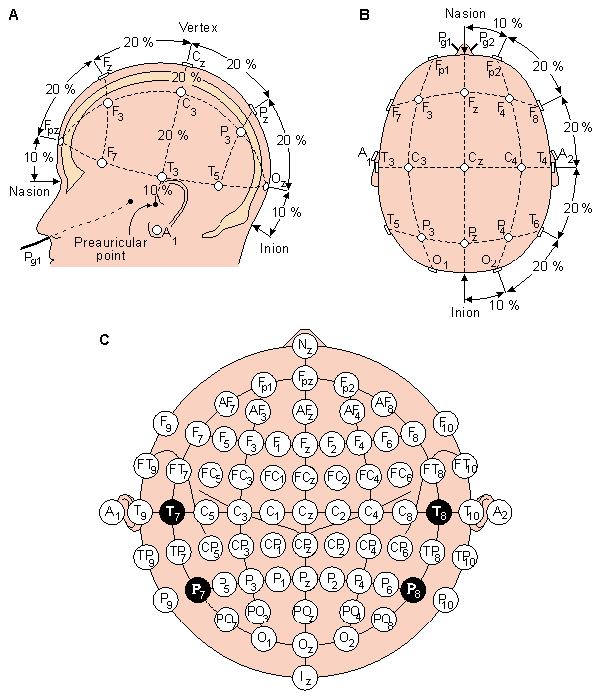
\includegraphics[scale=0.4]{obrazky/ElectrodePositions1020.png}
	\caption{The original 10-20 international system - internationally recognized method to describe and apply the location of scalp electrodes in the context of an EEG test or experiment. \cite{BCI2000}}
	\label{10-20}
\end{SCfigure}

\section{Data Sharing}

A trend toward increased sharing of neuroimaging data has emerged in recent years. Nevertheless, a number of barriers continue to impede easy sharing of experiment's data. Many researchers and institutions remain uncertain about how to share data or lack the tools and expertise to participate in data sharing. The use of \gls{edc} (Figure~\ref{stages-edc}) methods for neuroimaging greatly simplifies the task of data collection and has the potential to help standardize many aspects of data sharing. \cite{neuroinf} The motivation for sharing is:
\begin{itemize}
	\item \textbf{to accelerate progress in understanding of the brain}
	
	
	Several researchers claim that more rapid scientific discoveries are possible with shared data \cite{Milham2012} \cite{Poldrack2012}.
	\item \textbf{to improve data quality}
	
	The sharing data helps uncover mistakes as missing data, noise, errors, etc. and improves the quality of the data in the future experiments.
	\item  \textbf{to reduce cost of research} 
	
	Neuroimaging research is costly both in terms of the data acquisition costs and the time spent in data documentation. A significant amount of money could be saved from redundant data acquisition if data were shared with appropriate metadata descriptions. \cite{neuroinf}
\end{itemize} 

The situation is similar in electroencephalography. \cite{neuroinf} \cite{mrieeg}  \cite{incf_mission}


\begin{figure}
	\centering
	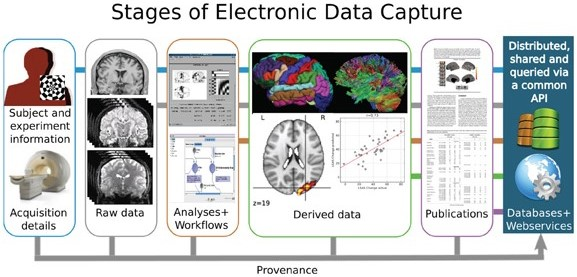
\includegraphics[scale=0.6]{obrazky/stages-EDC.jpg}
	\caption {Stages of Electronic Data Capture. \cite{neuroinf}}
	\label{stages-edc}
\end{figure}


\section{Program on Standards for Data Sharing}
\label{incf}
\gls{incf} Program on Standards for Data Sharing was established for the purpose of specification the standard for storing \gls{eeg} data. \gls{incf} is an international non-profit organization devoted to advancing the field of neuroinformatics and was established in 2005 in Stockholm. \gls{incf} community consists of 17 member countries and associated research groups, consortia, funding agencies and publishers in the field. The National Nodes are institutions or networks that represent each member country. The nodes are established to coordinate neuroinformatics activity within a country.  \cite{incfweb}

Program Standards for Data Sharing aims to develop generic standard and tools to facilitate the recording, sharing, and reporting of neuroscience metadata in order to improve practices for the archiving and sharing of neuroscience data. Metadata define the methods and conditions of data acquisition and subsequent analytical processing, Metadata also describe conditions under which the actual raw-data were acquired.

The current focus of the Program on Standards for Data Sharing is in two areas: neuroimaging and electrophysiology. \cite{incf_mission}. The most important requirement of such a standard is to accommodate common types of data used in electrophysiology or neuroimaging and also the metadata required to describe them. However we will focus on electrophysiology.

A standard way of storing metadata must be specified. The set of metadata required to describe electrophysiology data is difficult to determine a priori because the types of experiments are so varied.  A flexible mechanism must be used which allows referencing and specifying values for currently existing ontologies and also accommodates information not currently systematized. Techniques to include post-experiment annotations of data, and for relating different data parts, are also required. \cite{hdf5standard}

So far, the working group entertains two approaches towards defining a standard, which may eventually be merged. One, currently named Pandora, defines a generic data model that can be used with \gls{hdf5} or other storage back-ends. Due to the generic nature, the data model can be used to store various kinds of neuroscience data. The other proposal, called epHDF, defines domain specific schemata for storing electrophysiology data in \gls{hdf5}. \cite{hdf5standard}

The Electrophysiology Task Force of the \gls{incf} Program on Standards for Data Sharing is working on a document Requirements for storing electrophysiology data. The last version is 0.72 from 3rd November, 2014. This \gls{incf} internal document specifies all data that the standardized file format requires, defining what it must, should and may support. An overview of the stored data types is in Table~\ref{data_types}. \cite{requirements}
\begin{table}
	\begin{center}
		\begin{tabular}{|c|p{9cm}|}
			\hline Data type  & Description \\ 
			\hline Signal source & The origin of the recorded data; for example, the identity, position, etc. of the recording. This typically refers to information about a channel name, description, and location, or the target recorded.  There are at least two kinds of sources, including actors doing the recording (e.g. an electrode) and objects/actors being recorded (e.g. an subject, brain region, or neuron (real or putative))   \\ 
			\hline  Time series & An ordered collection of values given at defined points in time; for example, a recorded voltage  signal. It may correspond to raw data, recorded from “electrodes” or “channels”.   Alternatively, they could be derived from a data processing step.  The sampling may be done at regular time intervals (the sampling rate) or at irregular intervals (in which case a time point is required for each value).   \\ 
			\hline Signal events & The Signal events identify changes in a signal; for example, spikes, synaptic potentials, artifacts.  They could be raw data, for example, output of a hardware device that detects, and provides the times of spikes. They may also be generated as the result of processing data, for example, applying a spike detection algorithm on a time series signal. \\ 
			\hline  Image stacks & Image stacks are an ordered collection of images; the meaning of stack dimensions must be specified.  For example, a z-stack of images, a time series of images, a time-series of z-stacks, movies which are in standard formats.   \\ 
			\hline Experimental events & The Experimental Events data type consists of times of events, along with values that correspond to the times.   This data type can be used to describe: stimuli, trials or sweeps, time intervals, behaviors, and other events or conditions that occur during the experiment.   \\ 
			\hline Other / Generic array & Other data types and a mechanism for storing data types which have not been included in the standard. \\ 
			\hline 
		\end{tabular} 
		
		\caption{Overview of data types required by Requirements for storing electrophysiology data, Version 0.72. \cite{requirements}}
		\label{data_types}
	\end{center}
\end{table}






\section{Present formats for Storing \gls{eeg} Data}
Most known formats for storing \gls{eeg} data use the format \gls{hdf5}. Also both \gls{incf} proposals use \gls{hdf5} and the Electrophysiology Task Force of the INCF Program on Standards for Data Sharing in Requirements for a standard recommends basing a standard on \gls{hdf5}. \cite{requirements} Some formats are proprietary and even though some of them are well documented, is due to licenses complicated to use them or edit them. So I focus on the open ones. For storing \gls{eeg} neuroinformatics data many types of formats exist. The most known and used formats are Ovation \cite{ovation}, NeXus Format \cite{nexus}, NEO \cite{neo}, NeuroHDF \cite{neurohdf}, EDF+ \cite{kemp2003} and NIX (Pandora) \cite{pandora}. 

\subsection{Ovation}
Ovation is a commercial system for managing laboratory scientific data. The Ovation natively stores data in a database, but the data can be exported in \gls{hdf5} container. Ovation is cloud based data management and collaboration portal. It organizes files by projects and experiments while maintaining relationships between files and subjects, devices, and protocols used in experiment. \cite{ovation2} The description of the work model of Ovation is in Figure~\ref{ovation_work}. Although Ovation is a commercial system, the data model of Ovation is open \cite{ovation_m}. 

\begin{figure}
	\begin{center}
		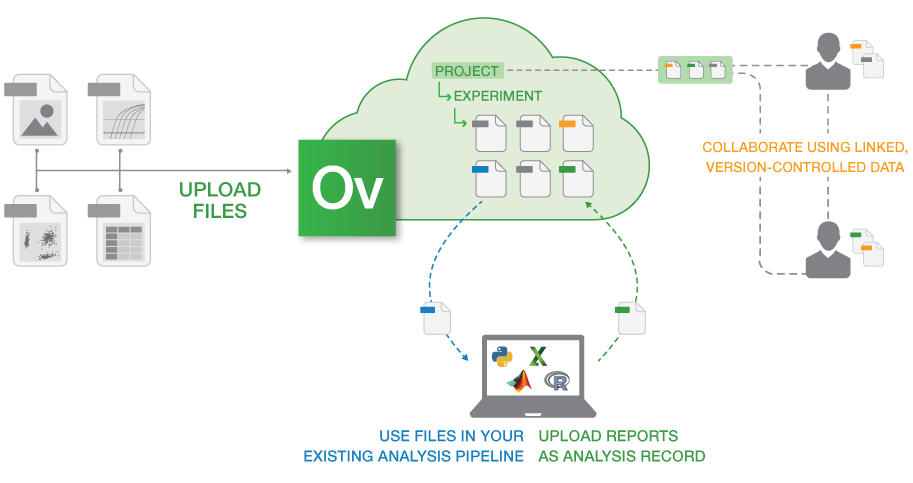
\includegraphics[scale=0.43]{obrazky/ovation.png}
		\caption{Ovation work model - Researchers upload their data into Ovation portal and describe them. Then they could work with data with existing analyze tools or work directly with project with linked version-controlled data. \cite{ovation2}}
		\label{ovation_work}
	\end{center}
\end{figure}

\subsection{European Data Format}
\gls{edf} is a format for storing multichannel biological and physical signals. This format has limitations for application in a field of evoked potentials, cardiology etc. A major limitation is that \gls{edf} can store only uninterrupted recordings. \gls{edf}+ was specified for that reasons. The EDF+ specification is incompatible with \gls{edf} only in allowing storage of several non-contiguous recordings. The \gls{edf} format support annotation for text, event and stimuli. An EDF and EDF+ data file consists of a header record followed by data records. The variable-length header record identifies the patient and specifies the technical characteristics of the recorded signals. \cite{edf} Information about signals, subject and whole measurements is defined and could not be changed. EDF+ format contains this information: version of format, patient identification (sex, birth date, subjects name), record identification (start date, start time, hardware identification, a code specifying the responsible investigator, a code specifying used equipment), number of data records, duration of records and number of signals in data record.


\subsection{NeXus Format}
\label{nexus_format}
NeXus is a format for data from Neutron and X-ray facilities. The format is also used for muon experiments. NeXus uses \gls{hdf5} as a default file container, but for compatibility reasons it is possible to use also \gls{hdf4} or \gls{xml} for special use cases. This format supports saving data and metadata into a single file. Several schemes are available for storing metadata sections, but the terminology is not defined and informations are stored in general structures as note, log, parameter or characterization. \cite{nexus}

\subsection{NEO}
Neo is a package for representing electrophysiology data in Python. This software package is able to load data from closed manufacturers' formats as Axon, Spike2, AlphaOmega, BlackRock and others. Neo implements a hierarchical data model and supports exporting to several neutral formats including \gls{hdf5}, MATLAB .mat file with NEO structure (NeoHDF5, NeoMatlab,.. ) or other open source tools WinEdr, WinWcp, PyNN, etc. The recommended way of use of this package is converting a closed format into more standard and open formats - NeoHDF5 or NeoMatlab. 



The goal of Neo is to improve interoperability between Python tools for analyzing, visualizing and generating electrophysiology data by providing a common, shared object model. In order to be as lightweight a dependency as possible, Neo is deliberately limited to presentation of data, with no functions for data analysis or visualization. Neo implements a hierarchical data model well adapted to intracellular and extracellular electrophysiology and \gls{eeg} data with support for multi-electrodes. \cite{neo}

\subsection{NeuroHDF}
This format also uses \gls{hdf5} as the main container for storing data. NeuroHDF is an effort to combine the flexibility and efficiency of \gls{hdf5} for neuroscience datasets through the specification of a simple layout for different data types with minimal metadata. \cite{neurohdf} 

\subsection{NIX}
\label{nixsection}
This format also uses \gls{hdf5} as a data container. This format specification closely defines an inner structure of file, especially the data part. The meta data part is defined by the \gls{odml}. 
The NIX project (previously called Pandora) started in the context of the Electrophysiology Task Force which is part of the \gls{incf} Datasharing Program. 

NIX is one approach to this problem: it uses highly generic models for data as well as for metadata and defines standard schemata for \gls{hdf5} files representing these models. Last but not least NIX aims to provide a convenient C++ library to simplify the access to the defined format. The design principle of the data model used by NIX was to create a rather minimalistic, generic, yet expressive model that is able to represent data stored in other widely used formats or models like Neuroshare or NEO without any loss of information. Due to its generic approach, the data model is also able to represent other kinds of data used in the field e.g. image data or image stacks. \cite{pandora}

\begin{figure}
	\begin{center}
		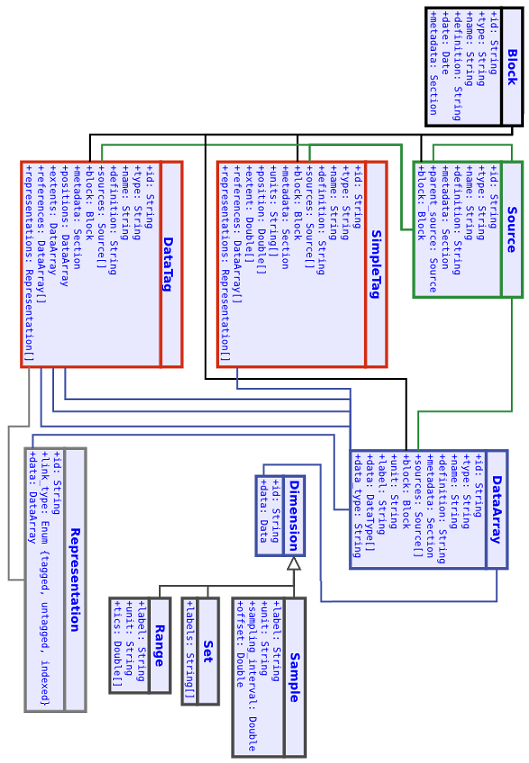
\includegraphics[scale=0.95]{obrazky/NIX_scheme.png}
		\caption{NIX data scheme. \cite{pandora}}
		\label{NIX_scheme}
	\end{center}
\end{figure}

This format's scheme (Figure~\ref{NIX_scheme}) was taken as inspiration for my file format, because it is discussed within the INCF Datasharing Program (Chapter~\ref{incf}) and it is recommended to use the file model of NIX. The measurements are stored in blocks. Each block identifies measurement and related metadata section. Raw data (signals, stimuli) are saved in DataArrays and they are specified by Dimension, Sample, Set, Representation and Range (Figure~\ref{NIX_scheme}) and could be specified by DataTag. The stimuli and artifacts are stored in SimpleTag (one stimulus) or MultiTag (more stimuli). The source of DataArrays or Tags could be specified by Source. Each section could contain link to the metadata part with measurement information. Closer description is available in Section~\ref{section_data}.



\subsection{epHDF}
This format is discussed within the \gls{incf} Program on Data Sharing standard. It uses \gls{hdf5} and deals with two issues. It is virtually impossible to anticipate all of the types of data and metadata that will need to be stored and no standard scheme exists for specifying how data in \gls{hdf5} files should be organized. \cite{ephdf}
To address both of these difficulties, a layered approach is proposed.  The first layer, which is called \gls{hdfds}, provides domain-independent conventions for specifying how the data in \gls{hdf5} files are organized. 
 Main features of \gls{hdfds} are as follows: 
\begin{itemize}
\item Enables associating external schemata to components of an \gls{hdf5} file in a manner similar to how name spaces in an XML file identify elements. 
\item Specifies locations and a format for storing arbitrary metadata in a \gls{hdf5} file. 
 \item Allows linking metadata to particular data parts within a file and to external files. \cite{ephdf}
\end{itemize}

The second layer builds on the conventions in \gls{hdfds} to specify schemata for storing basic electrophysiology data types.  It is called second layer \gls{ephdf}.  The data types defined in \gls{ephdf} (time series, time series segment, neural event and experimental event) are based on the entities defined in Neuroshare \cite{neuroshare} for covering the most commonly used data types in electrophysiology.  For each type, the data can be stored in whatever \gls{hdf5} numeric format is most efficient (for example 16 bit integer).  For all of the data types, a metadata schema is specified to include the fields needed to make a plot of the data with correct units. \cite{ephdf}

The epHDF for storing metadata uses \gls{odml}. An example of data annotation using \gls{odml} and \gls{json} encoding is bellow in listing~\ref{ephdf_example}. The listing shows description of amplifier hardware and its parameters. \cite{ephdf}
\newpage

\begin{lstlisting}[language=XML,label=ephdf_example,caption=Example of  data annotation using odML and JSON encoding.]
{
  "schema": "odml:hardware/amplifier.xml",
  "model" : <string_value>,
  "manufacture" : <string_value>,
  "serial_no" : <string_value>,
  "inventory_no": <string_value>,
  "owner" : <string_value>,
  "amplifier_type": <string_value>,
  "measurement_type": <string_value>,
  "operation_mode": <string_value>,
  "switching_frequence": <numeric_value>,
  "duty_cycle" : <numeric_value>,
  "gain" : <numeric_value>,
  "high_pass_cutoff" : <numeric_value>,
  "low_pass_cutoff" : <numeric_value>,
}
\end{lstlisting} 

\subsection{Brain Vision Format}

\gls{eeg} data at \gls{uwb} are recorded by BrainVision Recorder \cite{brainvision} (Figure~\ref{recorder}). This program records raw data and saves it to three files, which are described in the next chapter. 

The BrainVision Recorder does not allow natively recorded data in any other format. Most recordings consist of three files. The format of these files is defined in the BrainVision Recorder User Manual \cite{brainUserManual}:
\begin{itemize}
	\item \textbf{data file}
	\label{eeg}
	
	This is binary file which contains recorded values from recording device. The data are stored as double numbers.
	
	\item \textbf{vhdr file}
	\label{vhdr}
	
	This text file is Brain Vision Data Exchange Header File Version 1.0 and includes basic information about measurements. The format of the header file is based on the Windows INI format. It consists of various named sections containing keywords/values. The file stores basic information about measuring: coding, name of data file, name of marker file, number of channels, sampling interval in microseconds, information about binary format (IEEE\_FLOAT\_32) and information about channels (Channel number, channel name, resolution of unit, unit). The sample file of stored data and metadata is in listings~\ref{HeaderFile1} ~\ref{HeaderFile2} ~\ref{HeaderFile3} ~\ref{HeaderFile5} and table~\ref{HeaderFile4}. The sample file shows data saved in the EEGBase format.
	
	\item \textbf{vmrk file}
	\label{vmrk}
	
	This is Brain Vision Data Exchange Marker File, Version 1.0. The marker file is based upon the same principle of sections and keywords as the header file. This text file contains information about markers. The file stores marker number, type of the marker, description, position, size and channel number. The example of file is in Listing~\ref{vmrk_file}.
	
\end{itemize}


\lstset{aboveskip=3mm,
	belowskip=3mm,
	showstringspaces=false,
	columns=flexible,
	basicstyle={\small\ttfamily},
	breaklines=true,
	breakatwhitespace=true,
	tabsize=3,
	mathescape
}


\begin{lstlisting}[frame=single,caption={The header file example - Information about the file format.},label=HeaderFile1]
Brain Vision Data Exchange Header File Version 1.0
; Data created by the Vision Recorder
\end{lstlisting}
\begin{lstlisting}[frame=single,caption={The header file example - Information about coding, created files, data orientation, number of recorded channels and sampling interval.},label=HeaderFile2]
[Common Infos]
Codepage=UTF-8
DataFile=000007.eeg
MarkerFile=000007.vmrk
DataFormat=BINARY
; Data orientation: MULTIPLEXED=ch1,pt1, ch2,pt1 ...
DataOrientation=MULTIPLEXED
NumberOfChannels=48
; Sampling interval in microseconds
SamplingInterval=5000
\end{lstlisting}







\begin{SCfigure}[][h]
	\caption{Software used for EEG recording at University of West Bohemia - BrainVision Recorder. \cite{brainvision}}
	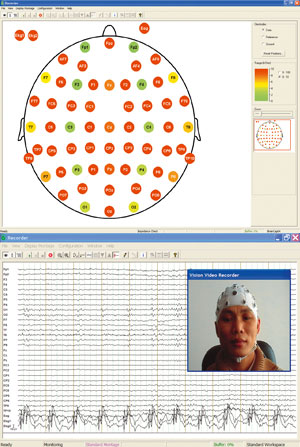
\includegraphics{obrazky/recorder.png}	
	\label{recorder}
\end{SCfigure}

\section{Hierarchical Data Format}

\gls{hdf} is a data model, file format and library for storing extremely large and complex data collections. \cite{hdf} This technology is able to store any kind of data and is used all over the world in research centers and government agencies. For example the format \gls{hdf5} is used by Cardiff University for resolving their problem with grid computing, Deutsche Bank for financial engineering, Diamond Light Source in synchrotron science (using NeXus format- Section \ref{nexus_format}), Laboratory for Neural Computation for bio-engineering and many others. A lot of formats for storing electrophysiology data use \gls{hdf5}. The adopters are able to solve variety of problems with \gls{hdf} format. (Figure~\ref{hdf_why}). 
"The grouping structure in \gls{hdf5} enables applications to organize data objects in \gls{hdf5} to reflect complex relationships among objects. The rich collection of \gls{hdf5} datatypes, including datatypes that can point to data in other objects, and including the ability for users to define their own types, lets applications build sophisticated structures that match well with complex data. The \gls{hdf5} library has a correspondingly rich set of operations that enables applications to access just those components that are important." \cite{hdf}


\gls{hdf} is similar to \gls{xml} documents, \gls{hdf} files allows to specify complex data relationships and dependencies and are self-describing. Several APIs for programing languages C, C++, Fortran 90, Java and others are available for this format. 
\gls{hdf} is open-source (\gls{bsd} license), stored data are human readable and the metadata model is easily customized.


\begin{figure}[h]
	\begin{center}
		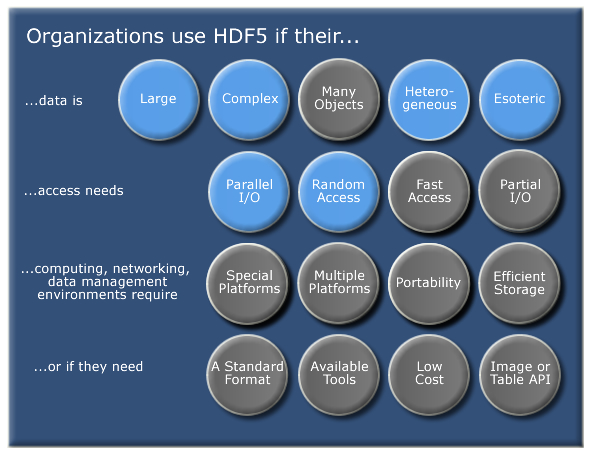
\includegraphics[scale=0.85]{obrazky/hdf_why.png}
		\caption{Detailed descriptions of some of the data challenges facing HDF adopters. \cite{hdf}}
		\label{hdf_why}
	\end{center}
\end{figure}

The advantages of using \gls{hdf5}: \cite{neurohdf}
\begin{itemize}
	\item \textbf{Compact binary data storage, extensible metadata}
	
	The \gls{hdf5} container could use software lossless compression. Szip and Gzip are a stand-alone libraries that are configured as optional filters in \gls{hdf5}. An Application is using Szip or Gzip compression when a dataset is created and if Szip (Gzip) encoder is enabled, data is automatically compressed and decompressed by Szip (an implementation of the extended-Rice lossless compression algorithm) or Gzip compression. (Figure~\ref{hdf_compression}). \gls{hdf5} allows to use third party compression filters too.
	
	
	\begin{SCfigure}
		\centering
			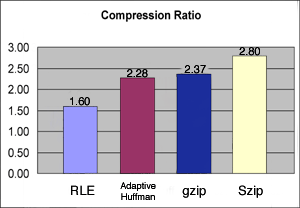
\includegraphics[scale=0.89]{obrazky/H4_szip_size.png}
			\caption{Comparison of compression performance in tests with HDF4. Size of compressed output with Szip in HDF4. The test were conducted with HDF4 format, but the compression algorithms are the same in HDF5.}
			\label{hdf_compression}
	\end{SCfigure}
	
	\item \textbf{Fast random and parallel access, efficient, scalable}
	
	The \gls{hdf} already supports parallel I/O and there is project of the European synchrotron particle accelerator community on developing the capability for multiple reader processes to read from an HDF5 file while another process writes to the file. The \gls{hdf} container supports compression.
	\item \textbf{Widely used in High Performance Computing}
		
	\item \textbf{Open source and cross-platform}
	
	The \gls{hdf5} format is open source and the HDF Group offers API in many languages (C, Java, Python, Fortran,..) for a various platforms.
	\item \textbf{Possible speed up the query} \cite{hdffast}
\end{itemize}
Possible limitations of \gls{hdf5}: \cite{neurohdf}
\begin{itemize}
	\item \textbf{Difficulty to store variable-length string properties.}
	
	Storing of string properties is not simple, especially for strings with variable length.
	\item \textbf{Deleting a dataset does not free the space on disk.}
	
	The deletion of a dataset from \gls{hdf5} file does not free the space and the dataset stays in the file (but is inaccessible). The release of the space on disk requires rewriting the file.

	\item \textbf{Evaluating \gls{hdf5}}
	
	There is no tool to evaluate \gls{hdf5} files. The \gls{hdf} allows storing of any data and it is complicated to evaluate it.
	\item \textbf{Delete or update a dataset in \gls{hdf5}} 
	
	The size of the dataset cannot be reduced after it is created. The dataset can be expanded by extending one or more dimensions, with function H5Dextend. It is not possible to contract a dataspace, or to reclaim allocated space.
\end{itemize}

\section{Ontologies}

Ontologies are formalized vocabularies of terms. Yann Le Franc defined ontologies this way: "Ontologies are formal models of knowledge in a particular domain and composed of classes that represent concepts defining the field as well as the logical relations that link these concepts together." \cite{ontology} The model of ontology is in Figure~\ref{ontology_scheme}.

\begin{SCfigure}[][h]
	\centering
	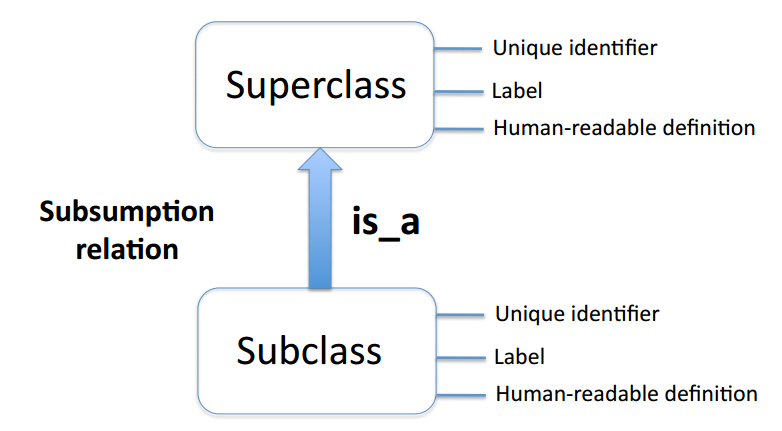
\includegraphics[scale=0.5]{obrazky/ontology.png}
	\caption{Ontology model. \cite{ontology}}
	\label{ontology_scheme}
\end{SCfigure}

\subsection{Neural ElectroMagnetic Ontology}
Neural ElectroMagnetic Ontology describes classes of event-related brain potentials and their properties, including spatial, temporal, and functional (cognitive/behavioral) attributes, and data-level attributes (acquisition and analysis parameters). \cite{nemo}
\subsection{Gene Ontology}
This project provides an ontology of defined terms representing gene product properties. 
The ontology covers three domains: cellular component, molecular function and biological process. \cite{bruha}
\subsection{Phenotype And Trait Ontology}
"Phenotype And Trait Ontology is an ontology of phenotypic qualities intended for use in a number of applications, primarily defining composite phenotypes and phenotype annotation, Phenotypic qualities (properties). This ontology can be used in conjunction with other ontologies." \cite{bruha}
\subsection{The Open Biomedical Ontologies Foundry}
The \gls{obo} Foundry is a collaborative experiment involving developers of science-based ontologies who are establishing a set of principles for ontology development with the goal of creating a suite of orthogonal interoperable reference ontologies in the biomedical domain. \cite{oen}
\subsection{OBO Relations Ontology}
Relations Ontology is a collection of relations intended primarily for standardization across ontologies in the \gls{obo} Foundry and wider \gls{obo} library. It incorporates core upper-level relations such as part of as well as biology-specific relationship types such as develops form. \cite{smith2005}
\subsection{NIFSTD}
\gls{nifstd} is a core component of \gls{nif} project, a semantically enhanced portal for accessing and integrating neuroscience data, tools and information. \gls{nifstd} includes a set of modular ontologies that provide a comprehensive collection of terminologies to describe neuroscience data and resources. \cite{nifstd}
\subsection{Basic Formal Ontology}
The \gls{bfo} is a small, upper level ontology that is designed for use in supporting information retrieval, analysis and integration in scientific and other domains. \gls{bfo} is a genuine upper ontology designed to serve data integration in scientific and other domains. Thus it does not contain physical, chemical, biological or other terms which would properly fall within the coverage domains of the special sciences.  \cite{bfo}
\subsection{Computational Neuroscience Ontology}
\gls{cno} is a controlled vocabulary of terms used in Computational Neurosciences to describe models of the nervous system. This first release of \gls{cno} is an alpha version and should be further aligned with other ontologies accessible on Bioportal and should be made compliant with the \gls{obo} foundry recommendations. \cite{cno}
\subsection{Ontology for Biomedical Investigations}
Ontology for Biomedical Investigations is an ontology of investigations, the protocols and instrumentation used, the material used, the data generated and the types of analysis performed on it. \cite{obi}


\section{Open Metadata Markup Language}

\begin{figure}[h]
	\begin{center}
		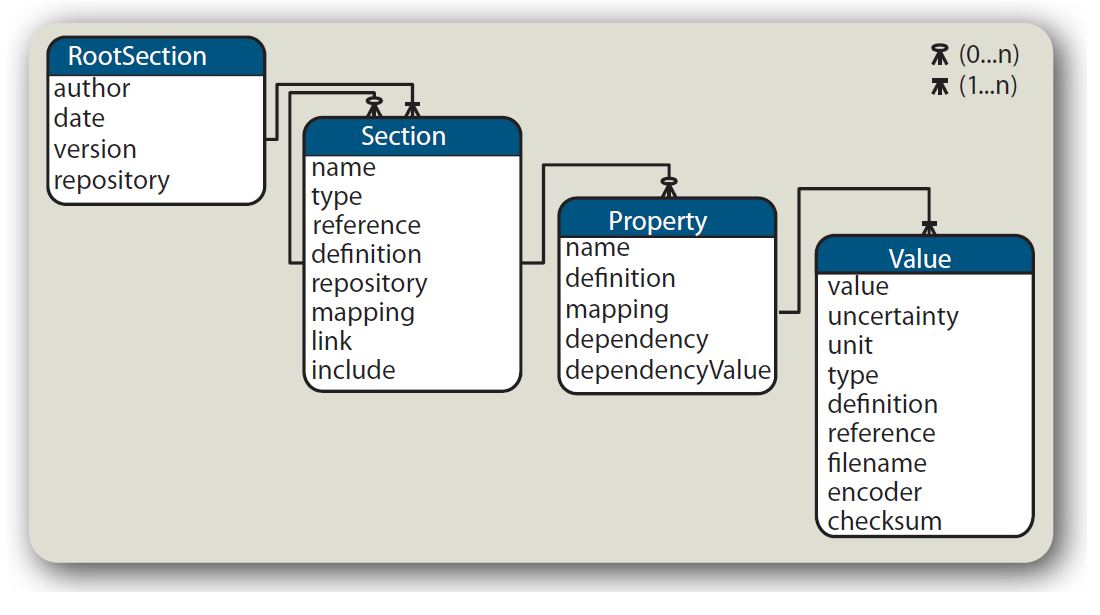
\includegraphics[scale=0.4]{obrazky/odml_tree.jpg}
		\caption{Open metadata Markup Language Entity-Relation diagram. \cite{odml}}
		\label{odml-tree}
	\end{center}
\end{figure}	
The metadata in electrophysiology domain providing information about stimuli, data acquisition, and experimental conditions are indispensable for the analysis and the management of experimental data within a lab. However, only rarely are metadata available in a structured, comprehensive, and machine-readable form. This poses a severe problem for finding and retrieving data, both in the laboratory and on the various emerging public data bases. \cite{odml} The \gls{odml} defines the format, not the content, so that it is inherently extensible and can be adapted to the specific requirements of any laboratory. For data sharing a correct understanding of metadata and data is only possible if the same terminology is used or if mappings between terminologies are provided. For this purpose were assembled terminologies with definitions of commonly used terms. \cite{odmlarticle}


\lstset{aboveskip=3mm,
	belowskip=3mm,
	showstringspaces=false,
	columns=flexible,
	basicstyle={\small\ttfamily},
	breaklines=true,
	breakatwhitespace=true,
	tabsize=3,
	mathescape
}
\begin{lstlisting}[language=xml,frame=single,label=odml_example,caption=Example of odml XML file.]
<?xml version="1.0" encoding="ISO-8859-1"?>
<?xml-stylesheet type="text/xsl" href="odmlTerms.xsl"  xmlns:odml="http://www.g-node.org/odml"?>
<!-- ********************************************************* -->
<!--                     Subject section                       -->
<!-- ********************************************************* -->
<odML version="1">
<repository>
http://portal.g-node.org/odml/terminologies/v1.0/terminologies.xml
</repository>
<version>1.0</version>
<date>2011-01-21</date>
<section>
<type>subject</type>
<name>Subject</name>
<definition>The investigated experimental subject (animal or person). May contain the Cell and Preparation sections as subsections.</definition>

<property>
<name>Comment</name>
<value>
<type>text</type>
</value>
<definition>A general comment on a specific subject. </definition>
</property>
\end{lstlisting} 



\gls{odml} stores data as extended key-value in hierarchical (tree) structure (Figure~\ref{odml-tree}). The main concept of \gls{odml} is to separate the content and the structure. The big benefit of \gls{odml} is that it is highly flexible and allows to save any kind of data.

"Property and Section entities are the core of the odml. A Section contains Properties and can further have subsection thus building a tree-like structure. The model further does not control the content which is a risk, on the one hand, but offers the flexibility." \cite{odml}. So far is the \gls{odml} model is implemented as a \gls{xml} schema. Listing~\ref{odml_example} shows the \gls{xml} file structure and provides example of \gls{odml} file.


\chapter {Analysis and Design}
The file format is divided into the two autonomous parts DATA and METADATA, which relate to each other, but could be read or written separately. The both parts are stored in one \gls{hdf5} container.

The data part stores all recorded binary data and the basic information about measuring for correct representation of measured data (Sampling interval, resolution and resolution unit). This section includes data from the eeg \ref{eeg}, vhdr \ref{vhdr} and vmrk \ref{vmrk} files. The file structure is defined by the NIX file model - (Figure~\ref{NIX_scheme}). I also use the same terminology and the file structure. However our model - EEGBase model was simplified for our needs. More specific description follows in Section~\ref{section_data}.

Java was selected as a programming language for program developing, because there is already parser of Brain Vision formats developed and also the EEGBase portal is written in Java. There is effort to include the export program into the EEGBase portal for easy export.



\section{Current Formats Comparison}
The comparison of the selected file formats is in Table~\ref{format_comparsion1}. Formats in the comparison were selected, because they use \gls{hdf5} and their model is open. The close models could be limited by licenses and their modifications could be limited.
The valuated criteria are: 
\begin{itemize}
\item \textbf{Proprietary} - the format is open source / closed
\item \textbf{Data terminology} - terminology for data (and necessary metadata) is defined
\item \textbf{Data ontology} - ontology for data is defined
\item \textbf{Metadata terminology} - terminology for metadata is defined
\item \textbf{Metadata ontology} - terminology for metadata is defined
\item \textbf{Portability} - the format has an \gls{api} for different languages, platforms
\item \textbf{Java API} - the format has Java \gls{api} (my program is in Java)
\item \textbf{Extensibility of model} - the data and metadata models are extensible
\item \textbf{Documentation of format} - the file format documentation and its availability
\end{itemize}
I evaluated formats with three grades compared to our needs. One is best, minus one is worst. The evaluation is subjective even though I tried to be as objective as possible.

\begin{table}[h]
	\caption{The current formats comparison.} 
	\scalebox{0.95}{
	\tabcolsep=0.13cm
	\begin{tabular}{| p{2,7cm} |c|c|c|c|c|c|c|}
		\hline \textbf{Format} &	\textbf{Ovation} 	& \textbf{EDF+} & \textbf{NeXus} & \textbf{NEO} & \textbf{neuroHDF} & \textbf{NIX} & \textbf{epHDF} \\ 
		\hline
		\hline Proprietary  	& -1 	& 1	 	& 1 & 1 & 1 & 1 & 1 \\ 
		\hline Data 
		
		terminology 		& 1 	& 1 	& 0  & 1 & 0 & 1 & 1  \\ 
		\hline Data 
		
		ontology 			& 1 	& 1 	& 0  & 1 & 1 & 1 & 1  \\ 
		\hline Metadata 
		
		terminology 		& 1 	& 1 	& -1  & 0 & -1 & 1 & 1  \\ 
		\hline Metadata 
		
		ontology 			& 1 	& 1 	& -1  & 0 & -1 & 1 & 1  \\ 						
		\hline Portability  & 0 	& 1 	& 1 & 1& 1 & 0 & -1  \\ 
		\hline Java API  	& -1 	& 1 	& 1 & -1  & -1 & -1 & -1\\ 
		\hline Extensibility & 0 	& -1 	& -1  & 0 & 0 & 1 & 1 \\ 
		\hline Documentation & 1 	& 1 	& 1  & 1 & 0 & 1 & 0 \\ 
		\hline 
		
	\end{tabular}  
}
\label{format_comparsion1}	
\end{table}

NIX and epHDF look like the best models. Both these models are supported by \gls{incf}.The NIX project offers only C++ \gls{api} and epHDF is only a standard for file format. Because my effort was integrate program for exporting measured data into the EEGBase portal \cite{eegportal}, which is in Java, I choose Java as the programming language for my program. The HDF Group provides Java \gls{api} for read and write \gls{hdf} files so I was able to create my own program that writes data in the \gls{hdf5} container. Because the NIX model is better commented and provides \gls{api}, I choose NIX as a initial solution for EEGBase format.

\section{Data Model}
\label{section_data}
The data model is based on the NIX data model (Figure~\ref{NIX_scheme} and Section~\ref{nixsection}). The NIX model is able to save data from any electrophysiology experiment. But for \gls{eeg} experiments the NIX model is too general. So I used only necessary parts of the model and other sections were omitted. The omitted parts are in the NIX model optional, so my format is compatible with the NIX definition. My data model is described in Figure~\ref{format_scheme}. The data model uses the NIX scheme of Block, DataArray, MultiTag, DataTag and SimpleTag. The Block is used to divide measuring, DataArray stores raw data of signals and stimuli and MultiTag stores stimuli information and DataTag contains \gls{eeg} channel information. DataArrays are divided for better distribution in my model to SIGNAL and MARKER parts. Also, the names of DataArrays correspond to names of channels. These adjustments allow better human readability and do not influence information or the model compatibility.

\begin{figure}
	\begin{center}
		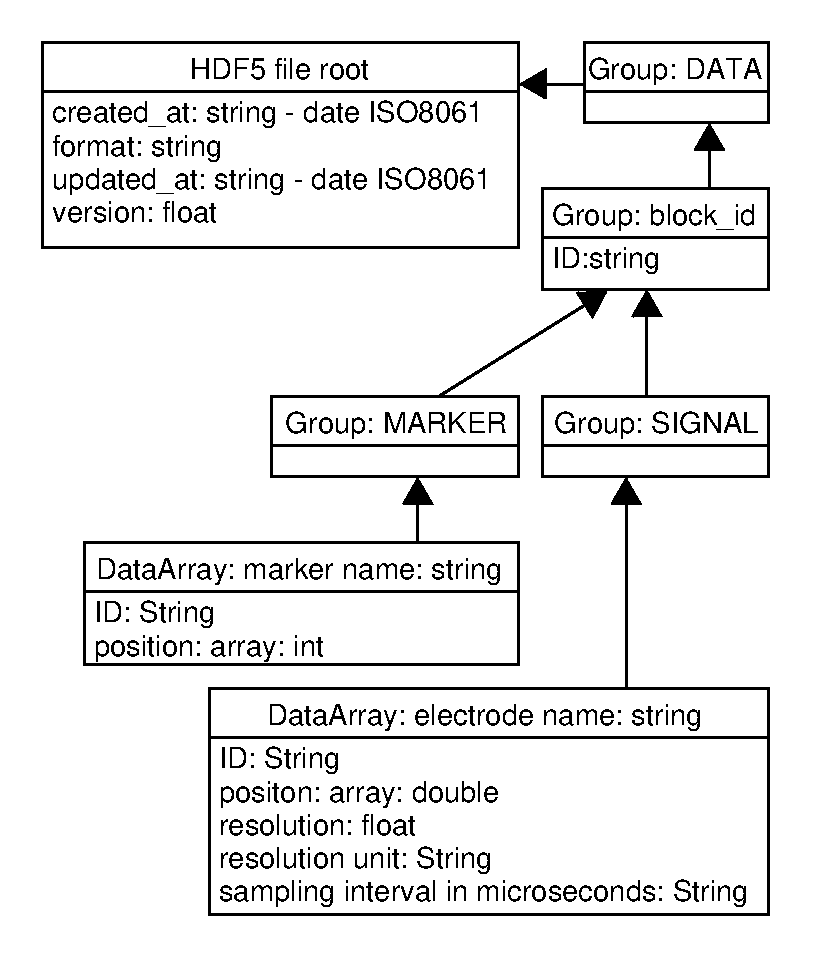
\includegraphics[scale=0.51]{obrazky/data.pdf}
		\caption{The final data model of proposed data format. The data are stored in tree structure with fixed terminology and structure. Each Group MARKER and SIGNAL could contain zero or more DataArrays with raw data.}
		\label{format_scheme}
	\end{center}
\end{figure}


\section{Model Ontology}
\subsection{Data Part}
Ontology and terminology of the data part is based on the NIX model that is described above in Section~\ref{section_data} - Data model and in Figure~\ref{format_scheme}.

\subsection{Metadata Part - odML}
\label{odml_section}
Metadata are organized according to \gls{odml} terminology. The \gls{gnode} \gls{odml} scheme and terminology was used for the metadata part of file, but there was some more information in the metadata scheme used at \gls{uwb}, which was difficult to save with existing \gls{odml} terminology. Therefore the \gls{odml} model and terminology were extended. The changes and adjustments are described in Section~\ref{meta_adjustments} - Metadata adjustments. We also decided that it would be useful to store some more data, which are more specific and could help to describe experiments better. The existing ontologies were also searched, for example Ontology for biomedical investigations \cite{oen} \cite{Brinkman2010}. However, I decided to use \gls{odml} because I was able to extend \gls{odml} to perfectly fit our needs and it is already used by the NIX model.


\subsection{UWB Metadata Model}
\label{meta_part}
This section shows all collected metadata, which are saved with experiments at \gls{uwb} and stored in the EEGBase portal \cite{eegportal}. The summary and comparison between the EEGBase portal information and original \gls{odml} (without our changes) model is in Table~\ref{comparsion}.

\newpage
\begin{longtable}{|l|l||l|l|}
	
\caption{The comparison between the EEGBase portal metadata model and terminology used by the odML model (without my adjustments).} \label{comparsion}\\
	\hline
	\multicolumn{2}{|c||}{\textbf{EEGBase}}& \multicolumn{2}{|c|}{\textbf{odML}} \\
	\hline 
	 \hline 
	\endfirsthead
	\multicolumn{4}{c}
	{\tablename\ \thetable\ -- \textit{Continued from previous page}} \\
	\hline	 
	\multicolumn{2}{|c||}{\textbf{EEGBase}}& \multicolumn{2}{|c|}{\textbf{odML}} \\
	\hline
	\hline  
	\endhead
	\hline \multicolumn{4}{c}{\textit{Continued on next page}} \\
	\endfoot
	\hline
	\endlastfoot
	 \hline Digitization & Gain & HW/Amplifier & Gain \\ 
	 \hline  Digitization & Filter & HW/Filter &  \\ 
 \hline 	 Digitization & Sampling\_rate & HW/DataAcq & SampleRate \\ 
 \hline 	 Pharmaceutical\footnote{Specification of pharmaceutics used by subject.} & Title & - &  \\ 
 \hline 	 Pharmaceutical & Description & - &  \\ 
 \hline 	 Artifact & Compensation & - &  \\ 
 \hline 	 Artifact & Reject\_condition	 & - &  \\ 
 \hline 	 Disease & Title & - &  \\ 
 \hline 	  Disease & Description & Subject & HealthStatus \\ 
 \hline 	 Weather & Description & - &  \\ 
 \hline 	 Weather & Title & - &  \\ 
 \hline 	 Artifact\_rem\_meth\footnote{Name of the used artifact remove method.} & Title & - &  \\ 
 \hline 	 Artifact\_rem\_meth\footnote{Description of the used artifact remove method.} & Description & - &  \\ 
 \hline 	 Software & Title & - &  \\ 
 \hline 	 Software & Description  & - &  \\ 
 \hline 	 Hardware & Title & HW/\textit{type}  & Model \\ 
 \hline 	 Hardware & Description &- &  \\ 
 \hline 	 Hardware & Type & - &  \\ 
 \hline 	 Project\_type & Title & Experiment & Type \\ 
 \hline 	 Project\_type & Description & - &  \\ 
 \hline 	 Subject\_group & Title &-  &  \\ 
 \hline 	 Subject\_group & Description & - &  \\ 
 \hline 	 Exper\_opt\_par\footnote{Name of optional experiment parameter.} & Param\_name & - &  \\ 
 \hline 	 Exper\_opt\_par\footnote{Data type of optional experiment parameter.} & Param\_type & - &  \\ 
 \hline 	 Exper\_opt\_par\_val\footnote{Value of optional experiment parameter.} & Param\_value & - &  \\ 
 \hline 	 Electrode\_conf & Impedance & Electrode & Impedance \\ 
 \hline 	 Electrode\_conf & Desc\_img\_ID & - &  \\ 
 \hline 	 Electrode\_system & Title & - &  \\ 
 \hline 	 Electrode\_system & Description & Electrode & ElectrodeCount \\ 
 \hline 	 Electrode\_location & Title & - &  \\ 
 \hline 	 Electrode\_location & Shortcut & - &  \\ 
 \hline 	 Electrode\_location & Description & - &  \\ 
 \hline 	 Electrode\_fix & Title & Electrode &  \\ 
 \hline 	 Electrode\_fix & Description & Electrode &  \\ 
 \hline 	 Electrode\_type & Title & Electrode & Type \\ 
 \hline 	 Electrode\_type & Description & Electrode &  \\ 
 \hline 	Scenario  & Title & - &  \\ 
 \hline 	Scenario  & Scenario\_Length & - &  \\ 
 \hline 	Scenario  & Description  & experiment/\textit{type} & Protocol \\ 
 \hline Scenario  & Scenario\_name & - &  \\ 
\hline Scenario  & Mimetype& - &  \\ 
\hline Stimulus & Description & Stimulus  & Desc/Start/End \\ 
	\hline Stimulus\_type & Description & - &  \\ 
	\hline Person & Givenname & Person & FirstName \\ 
	\hline Person & Surname & Person &LastName  \\ 
	\hline Person & Date\_of\_birth & Person & Birthday \\ 
	\hline Person & Gender & Person & Gender \\ 
	\hline Person & Email & Subject & ContactInfo \\ 
	\hline Person & Phone\_number & Subject & ContactInfo \\ 
	\hline Person & Note & Subject & Comment \\ 
	\hline Person & Laterality & - &  \\ 
	\hline Education\_level\footnote{Highest ducation level of person.} &Title  & - &  \\ 
	\hline Experiment & Start\_time & Recording & Start \\ 
	\hline Experiment &End\_time  & Recording & End \\ 
	\hline  Experiment& Temperature & - &  \\ 
	\hline  Experiment& Env\_note & - &  \\ 
	\hline  Experiment& Res\_group\_id & Recording & ExperimenterID \\ 
	\hline 
\end{longtable} 


\subsection{NIX Metadata Model}

The metadata model of NIX is using \gls{odml}. \gls{odml} is described in section \ref{odml_section}. The whole \gls{odml} terminology is too general and too extensive to list it here. So I chose the basic and most used sections which are related to our model and \gls{eeg} measurements and added it in Appendix~\ref{appendix1} in Figures~\ref{meta_scheme1}~\ref{meta_scheme2}~\ref{meta_scheme3}~\ref{meta_scheme4}. The EEGBase model contains modifications which are described below. 


\subsection{Metadata Terminology Extensions}
\label{meta_adjustments}
In order to save all our metadata into the \gls{hdf5} container I extended the \gls{odml} model for our metadata. These modifications were committed to \gls{gnode} respective \gls{incf} GitHub repository \cite{odmlgithub}. New sections \textbf{Environment}, \textbf{Protocol} and \textbf{Software} and several attributes to the existing sections \textbf{Person} and \textbf{Electrode} were added. All suggested changes were included into \gls{odml}. All modification are listed in Table \ref{modification}. Several attributes do not have descriptions, because their names are self-describing.
	\begin{longtable}{ | l | l | l | p{5cm} |}	
	\caption{Modifications of the \gls{odml} model.} 
	\label{modification}\\
\hline
\textbf{Name}& \textbf{Property} & \textbf{Value} & \textbf{Definition} \\
\hline 
\hline 
\endfirsthead
\multicolumn{4}{c}
{\tablename\ \thetable\ -- \textit{Continued from previous page}} \\
\hline	 
\textbf{Name}& \textbf{Property} & \textbf{Value} & \textbf{Definition} \\
\hline
\hline  
\endhead
\hline \multicolumn{4}{c}{\textit{Continued on next page}} \\
\endfoot
\hline

\endlastfoot
		Electrode & Usage & Ground & Usage of electrode. \footnote{Added terminology that describes usage of electrode.}\\
		\hline
		Electrode & Usage & Reference&Usage of electrode.\footnotemark[\value{footnote}] \\ 
		\hline
		Electrode & Usage & Channel& Usage of electrode.\footnotemark[\value{footnote}]\\ 
		\hline
		Electrode & Description & String& \\ 
		\hline		
		Environment & Weather & String & \\ 
		\hline	 
		Environment & RoomTemperature & String & \\ 
		\hline
		Environment & AirHumidity & float & The air humidity in \%.\\ 
		\hline
		Environment & Description & String &  \\ 
		\hline
		Protocol & Description & String & Description of the experiment\\ 
		\hline
		Protocol & Author & person & The persons who create this protocol.\\ 
		\hline
		Protocol & ProtocolFile & binary & Protocol File.\\ 
		\hline
		Protocol & ProtocolFileURL & URL & URL of protocol file.\\ 
		\hline
		Protocol & Version & String & Version of the protocol.\\ 
		\hline
		Person & Education level & String & Highest archived education level of the person.\\ 
		\hline
		Person & Role & Subject & The role of this person.\\ 
		\hline
		Person & Email & String & Person's e-mail.\\ 
		\hline
		Person & PhoneNumber & String & Person's phone number.\\ 
		\hline
		Person & Laterality & String & Handedness - The dominant hand of the subject.\\ 
		\hline
		Software & Name & String & The software name.\\ 
		\hline
		Software & Owner & String & The owner of software.\\ 
		\hline
		Software & Developer & String & Developer or developers firm of the software.\\ 
		\hline
		Software & Version & String & Version of the software.\\ 
		\hline
		Software & License & String & License type.\\ 
		\hline
		Software & LicenceStart & date & The start date of time limited license.\\ 		\hline
		Software & LicenceExpiration & date & The end date of time limited license.\\ 		\hline
		Software & LicenceDuration & String & Duration of the license for the software.\\ 		\hline
		Software & LicenceCount & int & Number of the software license.\footnote{For floating licenses}\\ 		\hline
		Software & Distribution & String & Distribution type.\\ 		\hline
		Software & Description & String & \\ 		\hline
		Software & LicenceDuration & String & Duration of the license for the software.\\ 		\hline
	\end{longtable} 

I also made some recommendations, which data would be useful to store a time zone, detail information about hardware and software and details about the project and experiments. The distribution of experiments by type in \gls{odml} is very useful and could be used in the EEGBase portal. The information about the project could be also helpful to identify a specific type of experiment. \gls{odml} is able to save most of these metadata and has a terminology for it so the EEGBase model is able to save them into the \gls{hdf5} container. When the current metadata model at University of West Bohemia will be extended it would not be problem to save it in EEGBase format. I suggested also that terminology of \gls{uwb} metadata model could use \gls{odml} terminology, because \gls{odml} have terminology for all currently saved information. 

\newpage
\subsection{EEGBase Metadata Model}
The model tree structure of EEGbase model metadata is in Appendix~\ref{appendix2}. Because \gls{odml} scheme is not mandatory but only recommended, it is possible to save, for example, experiments on mice which are also performed at \gls{uwb} in cooperation with The Faculty of Medicine - it is not necessary use both person and subject model, but it is possible to use only a subject's model. (Figure~\ref{person_vs_mouse}). The EEGBase model will store the tree structure of metadata into the EEGBase portal for easier, complete and adjustable metadata export.
\begin{figure}[h]
	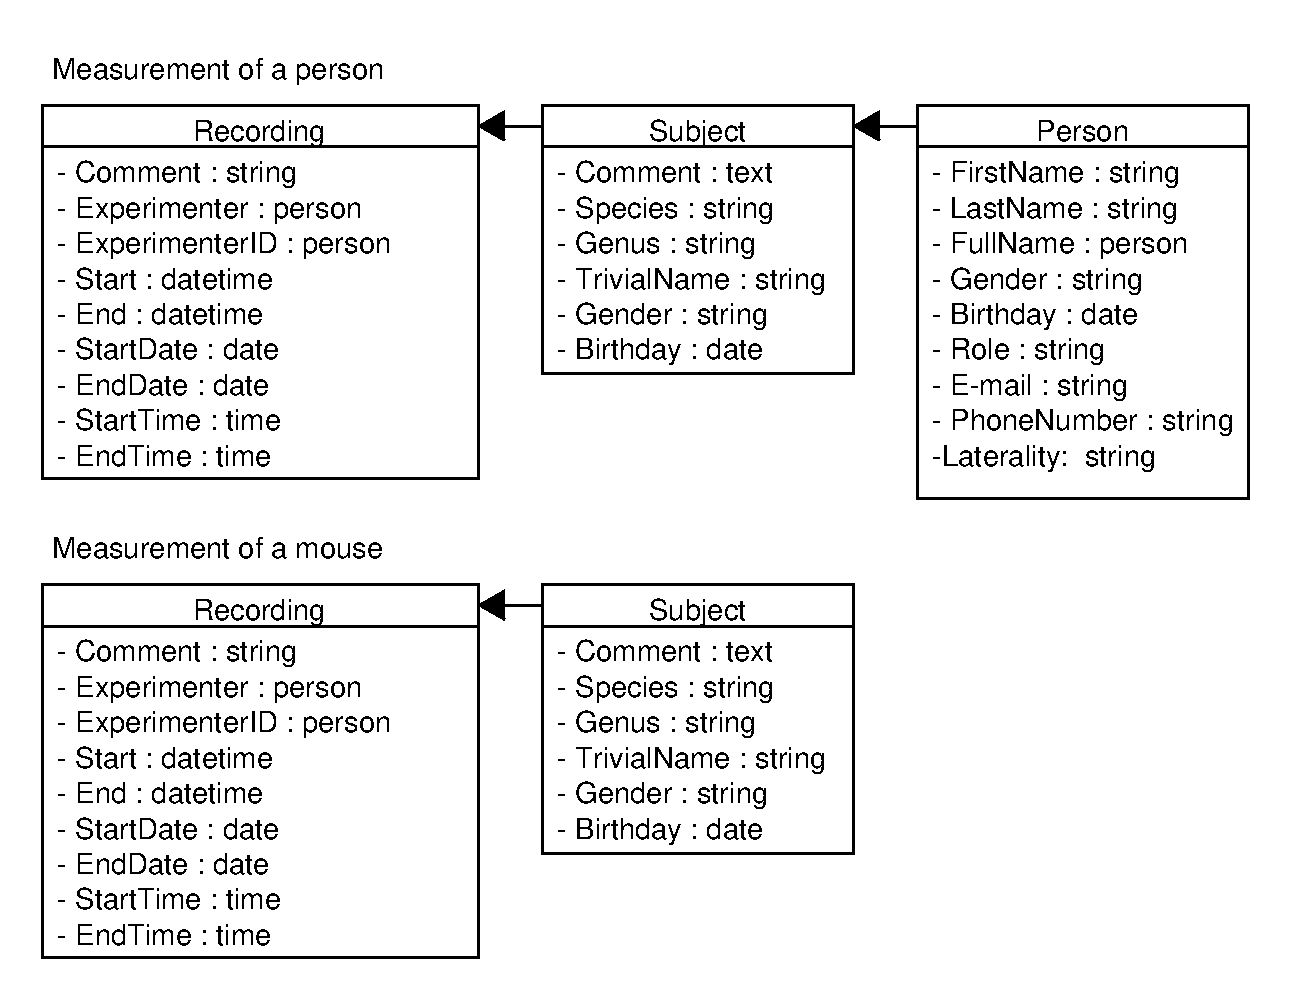
\includegraphics[scale=0.6]{obrazky/person_vs_mouse.pdf}	
	\caption{The comparison of metadata sections for saving experiments with a person or a mouse.}
	\label{person_vs_mouse}
\end{figure}
\newpage
\section{HDFExport Program}
\subsection{Program Specification}
I chose the Java programing language because I was hoping to implement this program as a part of the EEGBase portal so it will be possible to export the data directly from the portal through an internet browser. This approach is similar to what Ovation uses (store information in database and allows export to \gls{hdf5}). The problems with \gls{hdf} libraries came up. Closer information about the EEGBase portal integration is in Section~\ref{integration}. The other option was to create a desktop application that uses \gls{soap} web services of EEGBase portal for loading data and metadata for export.

The program is designed for several use cases divided by data and metadata location (Figure~\ref{use_case1}):
\begin{itemize}
\item data and metadata export from locally stored Brain Vision files only
\item data and metadata export from locally stored Brain Vision files and metadata from EEGBase portal
\item data and basic metadata export from in EEGBase postal stored Brain Vision files without experiments metadata
\item data and metadata export from EEGBase portal and Brain Vision files stored in EEGBase portal
\end{itemize}

\begin{SCfigure}
	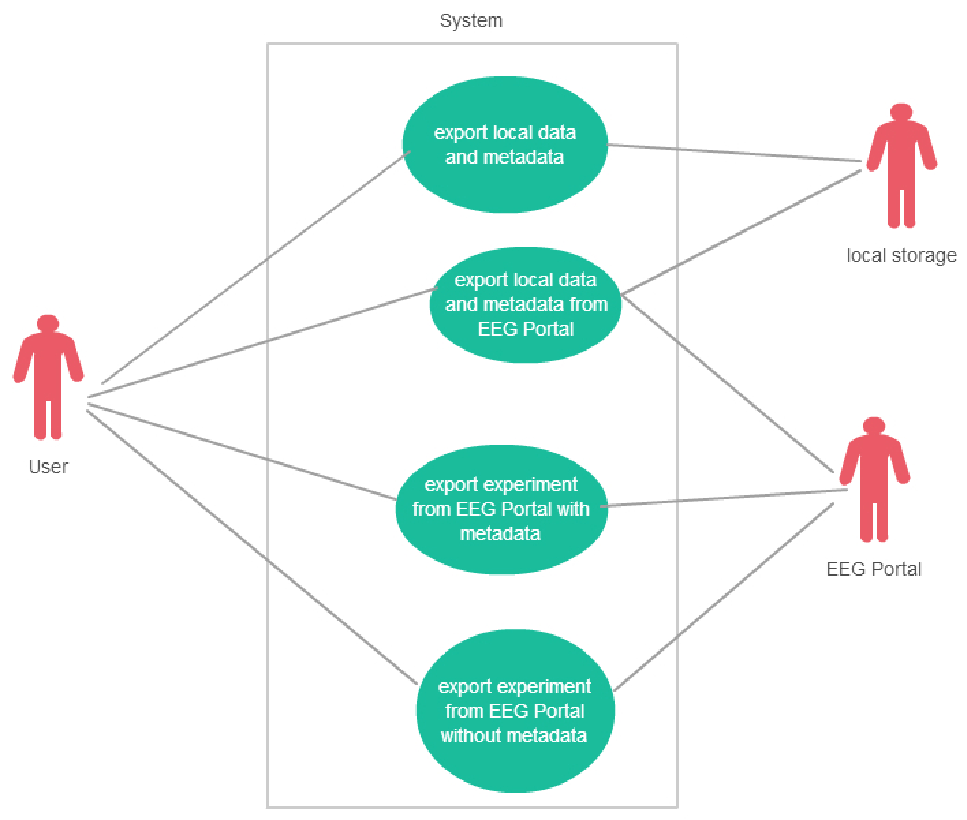
\includegraphics[scale=0.5]{obrazky/use_case_location.pdf}	
	\caption{Use cases of HDFExport Program.}
	\label{use_case1}
\end{SCfigure}
Other division is by type of exported data (Figure~\ref{use_case2}):
\begin{itemize}
	\item Only raw \gls{eeg} data and basic metadata are exported
	
	Only data and metadata from the Brain Vision files are exported. Stimuli are not exported (not all measurements uses stimuli).
	\item Raw \gls{eeg} data, basic metadata and stimuli are exported
	
	All data, metadata and stimuli from Brain Vision files are exported.
	\item Raw \gls{eeg} data, basic metadata, stimuli and experiments metadata are exported
	
	All data, metadata and stimuli from the Brain Vision files and experiments metadata from EEGBase portal are exported.
	\item Raw \gls{eeg} data, basic metadata and experiments information are exported
	
	All data, metadata and experiments information are exported.
\end{itemize}
\begin{SCfigure}
	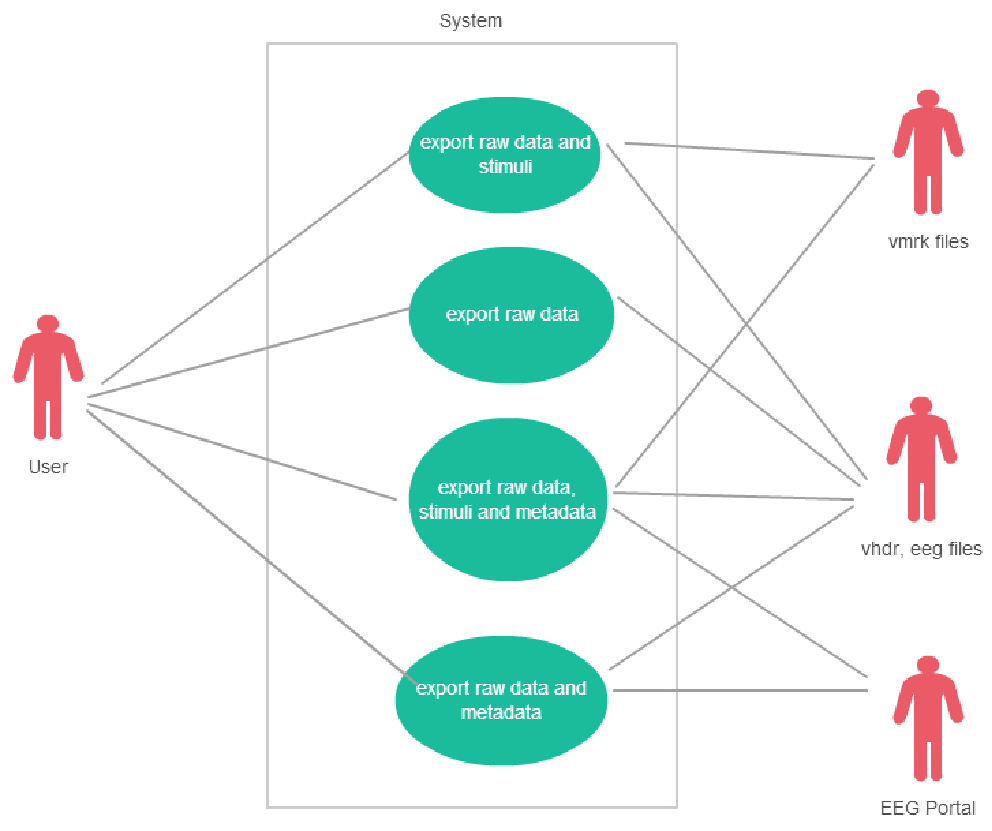
\includegraphics[scale=0.5]{obrazky/use_case_data.pdf}	
	\caption{Use cases of HDFExport Program.}
	\label{use_case2}
\end{SCfigure}


\begin{figure}[h]
	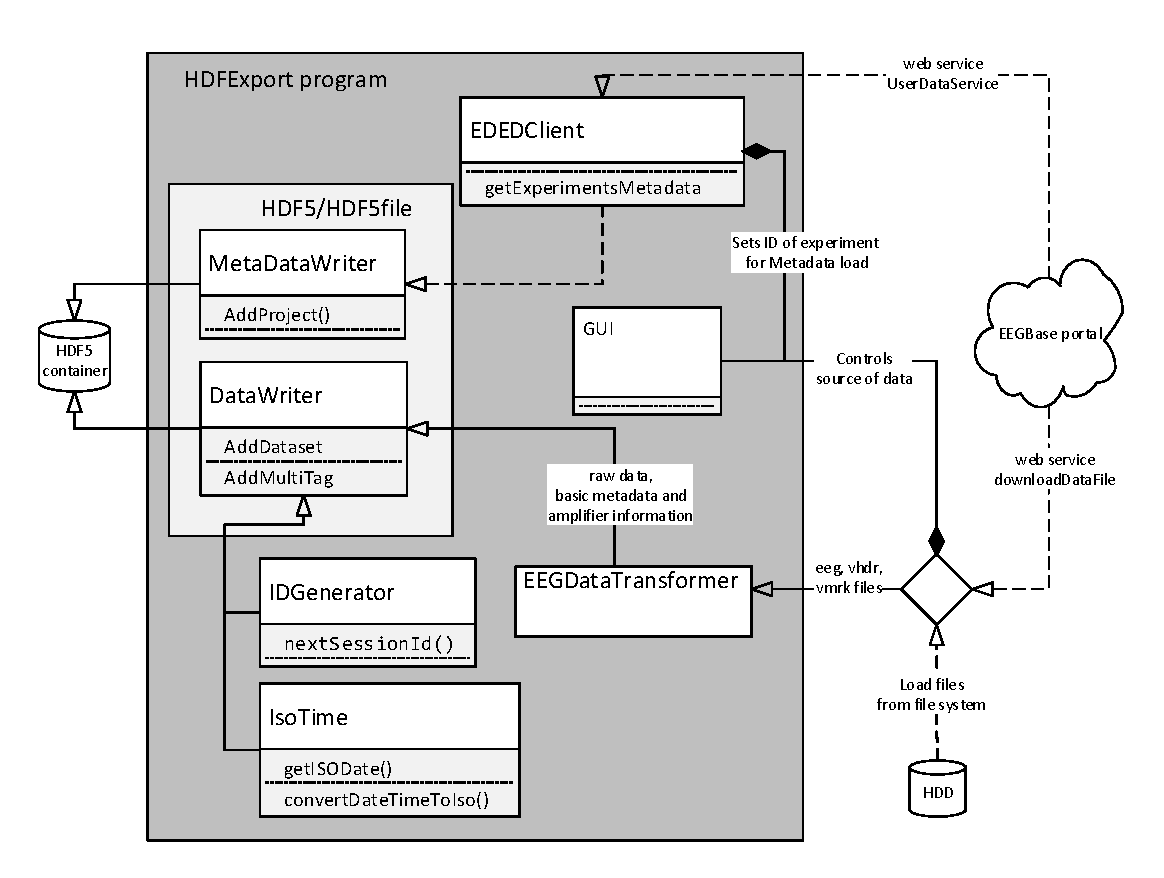
\includegraphics[scale=0.73]{obrazky/ExportProgramDiagram.pdf}	
	\caption{The diagram of EEGBase HDF5 export program}
	\label{export-diagram}
\end{figure}

\subsection{Architecture}
The program for export is based on the three layer architecture. The Brain Vision files parser (EEGDataTransformer), web service client (EDEDClient), HDF5 writer (uses HDF Group libraries for work with \gls{hdf5} container) and \gls{gui} are the most important parts of the program. Some supportive classes were written (IDGenerator, IsoTime). These generate unique IDs and date in ISO format.



\chapter{Implementation}
This chapter describe the EEGBase format implementation and the EEGBase Export program implementation. 

\section{HDF Libraries}
\label{hdflib}
This section explains which libraries and \gls{hdf5} structures I used for \gls{hdf} file operation. 

The disadvantage is that the NIX project has no Java \gls{api} so it was necessary to use the \gls{hdf5} Java \gls{api} \cite{hdfjava}, but this \gls{api} is not native. The HDF Group creates several libraries for Java. The HDF-Java wrappers consist of the Java \gls{hdf} Object Package, related \gls{hdf4} and HDF5 Object Packages, and the native \gls{jhi} and \gls{jhi5}. The native interface includes the Java classes and C interface libraries.

The most intuitive way is using the HDF Object Package \cite{hdf_object}. But I wrote my application with \gls{jhi5} which is used by HDF Object Package, because it calls directly native C functions. Therefore the program should be more quick and also more examples are available (the Java functions are similar to C and Python functions). 

"The HDF Object Package does not provide a one-to-one mapping from Java methods to routines in the standard \gls{hdf4} and \gls{hdf5} libraries. The one-to-one mappings are provided via the HDF Java Native Interface products \gls{jhi} and \gls{jhi5}. The HDF Object Package wraps these direct mappings with a higher level object model." \cite{hdf_object} The diagram is in Figure~\ref{hdf-obj}.

\begin{SCfigure}
	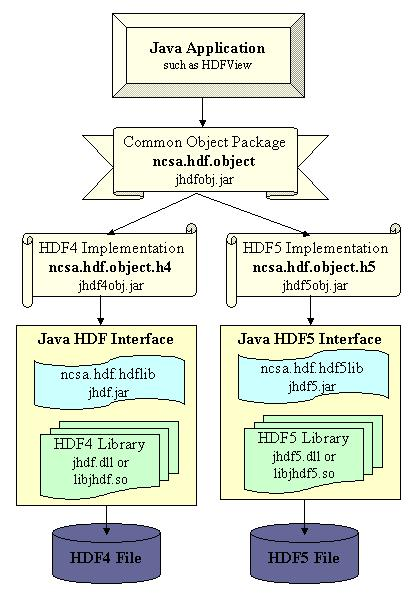
\includegraphics[scale=0.49]{obrazky/hdf-obj.jpg}
	\caption{The HDF Object Package. \cite{hdf_object}}
	\label{hdf-obj}
\end{SCfigure}

The \gls{hdf} works with five basic types of objects:

\begin{itemize}
	\item \textbf{Group}
	
A group is used as a folder in the file system, it divides objects into the logical groups. The group can contain none or more objects and can be member of another group.
\newpage
	\item \textbf{Dataspace}
	
This is a required part of \gls{hdf5} Dataset or Attribute. The Dataspace contains raw data and defines size and shape of data (defines the number of dimensions and size of each element).
	\item \textbf{Dataset}
	
	The Dataset is an object that describes stored data. It could contain none or more attributes and it is composed from raw data, metadata, data layout or other information necessary to write, read or interpret the stored data. The application view of a dataset is in Figure~\ref{dataset_figure}.	
	\begin{figure}[h]
		\begin{center}
			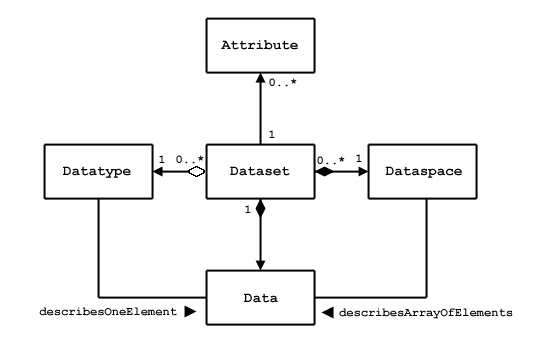
\includegraphics[scale=0.6]{obrazky/dataset.jpg}
			\caption{Application view of a dataset. \cite{hdf}}
			\label{dataset}
		\end{center}
	\end{figure}
		\begin{figure}[h]
			\begin{center}
				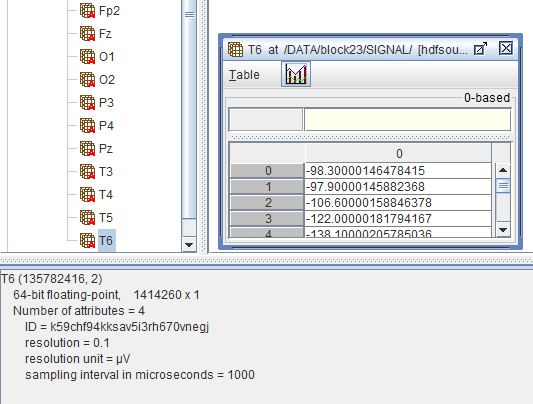
\includegraphics[scale=0.7]{obrazky/dataset-with-att.PNG}
				\caption{Example of HDF5 file with EEGBase format in HDFView 2.11- the Dataset with name T6 (EEG channel) with Dataspace (array of 1414260 double numbers) and four attributes.}
				\label{dataset_figure}
			\end{center}
		\end{figure}
	\item \textbf{Datatype}
	
The \gls{hdf5} datatype defines the storage format for a single data element. The description is in Figure~\ref{datatype}. The datatype describes the storage layout of a single data element. All elements of the dataset must have the same type and the datatype of a dataset is immutable.
	\begin{figure}[h]
	\centering
		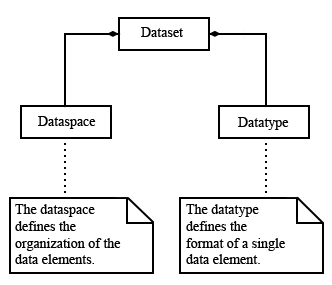
\includegraphics[scale=0.7]{obrazky/datatype.jpg}
		\caption{Datatypes, dataspaces, and datasets. \cite{hdf}}
		\label{datatype}	
\end{figure}

\newpage
	\item \textbf{Attribute}
	
	An \gls{hdf5} attribute is a small metadata object describing the nature and/or intended usage of a primary data object. A primary data object may be a dataset, group. Even though an attribute is not a standard \gls{hdf5} Dataset, it has several common properties: \cite{hdf}
	\begin{itemize}
\item An attribute has a user-defined dataspace and the included metadata has a user-assigned datatype
\item Metadata can be of any valid HDF5 datatype
\item Attributes are addressed by name
	\end{itemize} 
	Attributes are from Datasets different in:
		\begin{itemize}
			\item There is no provision for special storage such as compression or chunking
			\item There is no partial I/O or sub-setting capability for attribute data
			\item Attributes cannot be shared
			\item Attributes cannot have attributes
			\item Attributes are stored in the object header
		\end{itemize} 
\end{itemize}

Since all elements defined in \gls{hdf5} have names, they can be referenced by their path. \cite{pandora2}

\section{Used HDF5 Data Types}

The following data types were used in the \gls{hdf5} container:

\begin{itemize}
	\item \textbf{double} 
	
	The signal raw data are stored as the \gls{hdf5} type H5T\_IEEE\_F64LE.
	\item \textbf{float}
	
	Float numbers are saved as the \gls{hdf5} type H5T\_IEEE\_F32LE. The stimuli raw data are saved in this format.
	\item \textbf{string} 
	
	All strings are stored as type H5T\_C\_S1. Almost all attributes, dates and IDs are saved as strings.
	
\end{itemize}

\section{EEGBase File Structure}

The root of the file contains basic information about the file and the format. It also divides the file container into two groups Data and Metadata. (Table~\ref{file_root}). The \gls{iso} 8601 format was used for the date, because even though \gls{hdf5} has a data type for the date, it is not platform independent. The NIX model does not have the date format specified so I chose the norm of \gls{ecsn} \gls{iso} 8601 \cite{iso8601}, which is one of many possible formats and it is the Czech version of the international format \gls{iso} 8601:2004. This norm allows the user to save date and time at once and specify even the time zone. This could be important for the flawless representation of measured data. Then the final Date string is: Complete date plus hours, minutes, seconds and a decimal fraction of a second YYYY-MM-DDThh:mm:ss.sTZD (e.g. 1997-07-16T19:20:30.45+01:00) \cite{iso8601}. This date and time is saved as String so it is platform independent and thanks to the \gls{iso} norm is standardized.


Recordings are wrapped into the blocks (HDF groups). Each recorded channel with basic metadata is saved in a block. The recorded signal values (raw data) are stored in the Dataset with the name of the channel. Information from files eeg (Section~\ref{eeg}) (raw data) and vhdr (Section~\ref{vhdr}) (metadata) and generated IDs are stored in the DATA section.
Markers (stimuli and artifacts etc.) information are stored in a block in the section MARKERS and they are saved also in the Datasets with the name of the marker. (Figure~\ref{datasection_exp}).
\begin{table}
	\begin{tabular}{l l l}
		root &  & \\ 
		\hline attribute & format & string \\ 
		attribute & version & string \\ 
		attribute & created\_at & string - date ISO 8601 \\ 
		attribute & updated\_at & string - date ISO 8601\\ 
		\hline	 group &  DATA & \\ 
		group & METADATA & \\ 
		\hline	 
	\end{tabular} 
	\caption{The root of \gls{hdf5} file.} 
	\label{file_root}
\end{table}

\begin{SCfigure}[][h]
		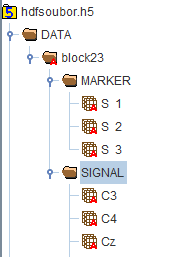
\includegraphics[scale=0.8]{obrazky/data-section.png}
		\caption{Example of HDF5 file with EEGBase format in HDFView 2.11- the DATA section.}
		\label{datasection_exp}

\end{SCfigure}

The \gls{hdf5} container stores information about array dimensionality and a stored data type natively. (Figure~\ref{dataset_figure}).

\section{HDFExport Program Modules}

\subsection{Brain Vision Files Parser}
The EEGDataTransformer from Jan Štěbeták \cite{eegloader} was used as a parser for current eeg, vhdr and vrmk files.  Only minor changes of this program were made. I added the class AmplifierInfo and ImpedanceInfo and the methods NumberOfChannels, SamplingInterval, getAmplifier, getImpedanceInfo into DataTransformer interface. The method getUnits() of ChannelInfo class was edited, because the returned String was in wrong format. Figure~\ref{eegexport}.

\begin{figure}
	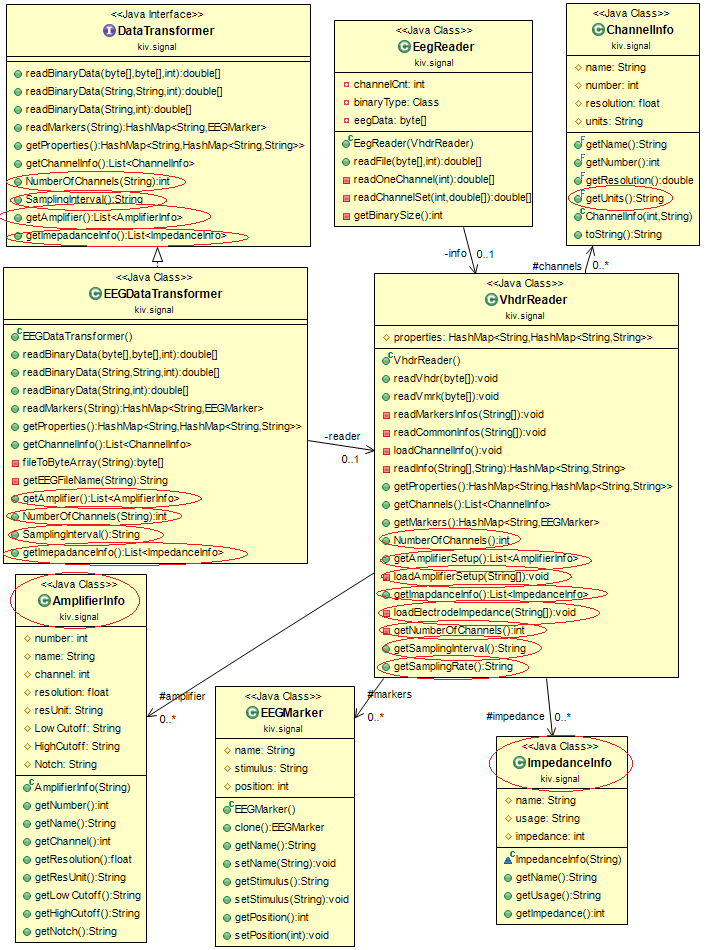
\includegraphics[scale=0.75]{obrazky/EEGExport.png}
	\caption{Class diagram of edited EEGDataTransformer program. New methods and classes are marked.}
	\label{eegexport}
	
\end{figure}

\subsection{Metadata Loader}
The metadata are loaded through web services, which were written by Jan Štěbeták \cite{webservice}, and from Brain Vision vhdr file.

The program uses the web service UserDataService and its methods for loading all experiments metadata.
The client was generated from \gls{WSDL} file \cite{wsdl}. EDEDCLient \cite{jerpa} written by Petr Miko was used as a client for web services.

\subsection{HDF5 Writer}
The writer consists of three classes:
\begin{itemize}
	\item HDF5file
	
	The the \gls{hdf5} file is created in this class and all necessary information about format (Version, Format name, Date) are written in the file. This class uses and calls methods from DataWriter and MetaDataWriter classes.
	
	\item DataWriter
	
	This class saves all binary data and markers to the \gls{hdf5} container. This class saves also essential metadata of raw data into attributes.
	
	\item MetaDataWriter
	
	This class stores all loaded metadata into METADATA part (Section~\ref{meta_part}).
	
\end{itemize}

\begin{figure}
	\begin{center}
		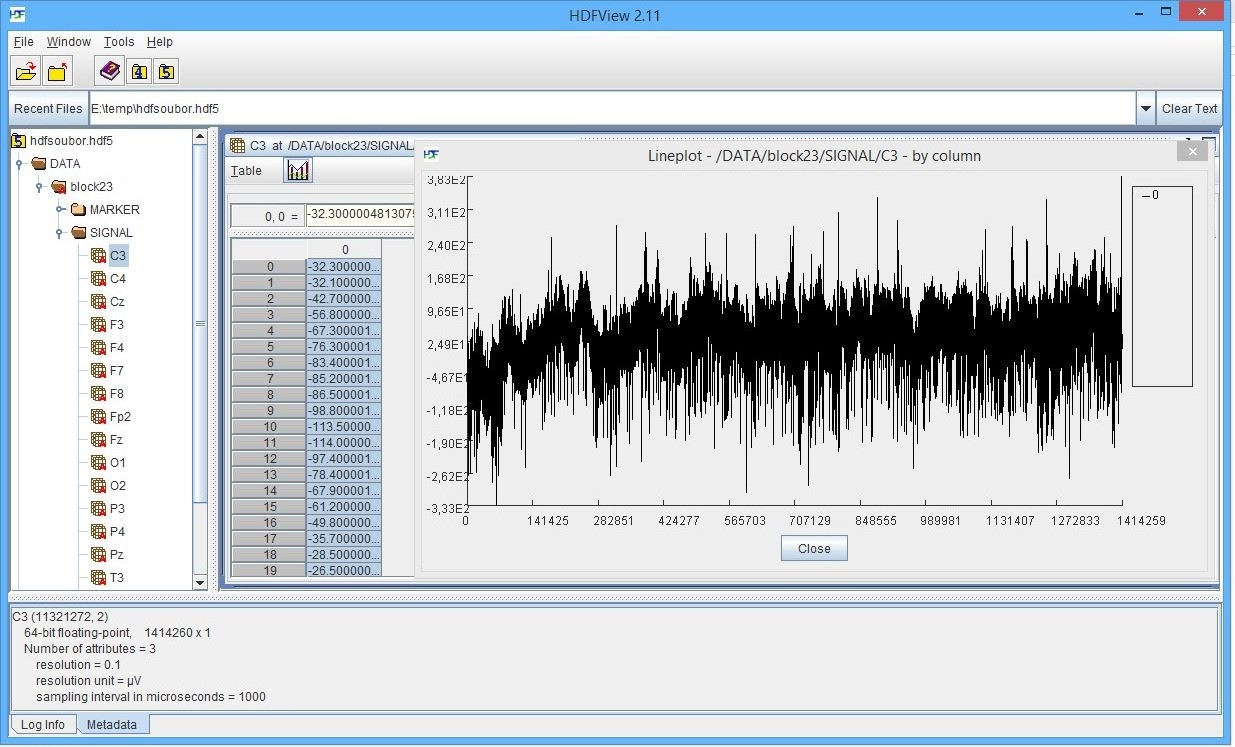
\includegraphics[scale=0.4]{obrazky/HDF5_file.jpg}
		\caption{HDF5 file with data with EEGBase format - in HDFView 2.11}
		\label{hdf5_file}
	\end{center}
\end{figure}

The programming was not simple, because the C methods stayed the same and the wrappers only allow to be called from Java Virtual Machine. The example of the Java code and calls of C functions are in Listing~\ref{java2}.
The methods for easier work with \gls{hdf5} libraries were written and the code for saving string into the \gls{hdf5} file is in Listing~\ref{stringsave} and for storing binary data into the datasets is in Listing~\ref{java3}.

\definecolor{dkgreen}{rgb}{0,0.6,0}
\definecolor{gray}{rgb}{0.5,0.5,0.5}
\definecolor{mauve}{rgb}{0.58,0,0.82}

\lstset{frame=tb,
	language=Java,
	aboveskip=3mm,
	belowskip=3mm,
	showstringspaces=false,
	columns=flexible,
	basicstyle={\small\ttfamily},
	numbers=none,
	numberstyle=\tiny\color{gray},
	keywordstyle=\color{blue},
	commentstyle=\color{dkgreen},
	stringstyle=\color{mauve},
	breaklines=true,
	breakatwhitespace=true,
	tabsize=3
}
\newpage
\begin{lstlisting}[language=C,frame=single,caption={Creating Group in HDF5 with Java wrappers. This code creates a new group with the name METADATA at the specified location block},label=java2]
//create Group
H5.H5Gcreate(this.block, "METADATA", HDF5Constants.H5P_DEFAULT, HDF5Constants.H5P_DEFAULT, HDF5Constants.H5P_DEFAULT);

\end{lstlisting}

\begin{lstlisting}[language=C,frame=single,caption={Saving binary data into the dataset. It saves H5T\_IEEE\_F64LE (double) in dset\_data if saving location dataset\_id exists},label=java3]
if (dataset_id >= 0) // location exists
H5.H5Dwrite(dataset_id, HDF5Constants.H5T_IEEE_F64LE, HDF5Constants.H5S_ALL, HDF5Constants.H5S_ALL, HDF5Constants.H5P_DEFAULT, dset_data);
\end{lstlisting}

\begin{lstlisting}[language=C,frame=single,caption={Saving string as attribute in HDF5.},label=stringsave]
//SaveString method
int attribute_space,attribute_id=-1;
int stype =-1;
//create space for one char
attribute_space = H5.H5Screate(HDF5Constants.H5S_SCALAR);
//copy size of char
stype = H5.H5Tcopy(HDF5Constants.H5T_C_S1);	
//sets size of string lenght*size of char
H5.H5Tset_size(stype, savedString.length());
//create attribute in location dataset_id, with name HdfName, size stype
attribute_id = H5.H5Acreate(dataset_id, HdfName, stype, attribute_space, HDF5Constants.H5P_DEFAULT, HDF5Constants.H5P_DEFAULT);
//writes string into prepared attribute_id, with size of stype
H5.H5Awrite(attribute_id, stype, savedString.getBytes());	
//if all was correct close space	
if(attribute_space>-1){
  H5.H5Sclose(attribute_space);
}
//if all was correct close attribute	
if(attribute_id>-1){
  H5.H5Aclose(attribute_id);
}

\end{lstlisting}




\subsection{Graphical User Interface}
The program has only a basic \gls{gui}, because the main purpose is to provide methods for saving all current data and metadata to the \gls{hdf5} container. The methods which are working with \gls{hdf5} container are general and it is possible to use them in any other program. All methods are in separate classes in a special package hdf5. \gls{gui} for locally stored data use case is presented in Figure~\ref{program-gui}.

\begin{figure}[h]
	\begin{center}
		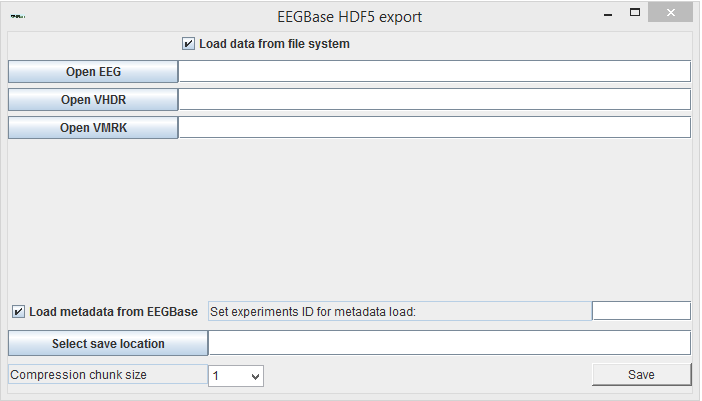
\includegraphics[scale=0.7]{obrazky/program_gui2.PNG}
		\caption{EEGBase HDF5 export program. Metadata are loaded trough web services.}
		\label{program-gui}
	\end{center}
\end{figure}

\section{EEGBase Portal Integration}
\label{integration}
Although my first effort was to import my program into the EEGBase portal, I was unable to do so. I tried to create a prototype which would save stored data into the \gls{hdf5} file in a web container. However I could not make Java wrappers work in the web container. I contacted \gls{hdf} Group support for advice, however, the support and developers did not know how to develop such a program. I did some research and I tried to make the program work on the Tomcat server and Glassfish server but with no success. For those reasons I chose to use the EEGBase portal \gls{soap} web services to load data for export to the \gls{hdf5} container.

It was necessary to create a new web service, which will export all metadata of the experiment. The web service \textit{getExperimentsMetadata} was created for that reason and it is used by my program.


\chapter{Tests}

The program was manually tested for several use cases and all created \gls{hdf5} files were verified manually (opened and the contents was checked) by official program of HDF Group HDFView \cite{hdfjava} in version 2.11 - Figure~\ref{hdf5_file}. The following test describing writing speed into \gls{hdf5} container were conducted. (Table~\ref{speed_test}). The file size of created files were also tested. (Table~\ref{file_size}).



\section{Performance Tests}

The write performance tests were conducted to determine time consumption of export. The tests were conducted on a standard desktop computer (processor Intel Core i7 at 3,4 GHz, 8 GB of DDR3 RAM, standard HDD with 7200 rpm). An unusually high memory consumption was detected during the test. The amount of occupied memory by the EEGExport program for big (220 MB) measurements reached up to 4 GB of memory. Further testing showed that Java Virtual Machine, in attempt to speed up export, does not free allocated memory. However, if the program was paused the amount of allocated memory was lower; the program could run with less memory. In the end the disk writing speed was a limited factor. The conversion times with GZip compression are shown in Table~\ref{speed_test}.

\begin{table}
	 \catcode`\-=12
	\centering
	\caption{Performance tests with GZip compression. Each file was saved seven times.}
	\label{speed_test}
	\begin{tabular}{|c|c|c|c|c|}
		\hline
\textbf{File size} & \multicolumn{4}{c|}{\textbf{Time needed for conversion in ms}}\\ 
	\cline{2-5}		
	\textbf{ of Brain Vision files}	&\textbf{Best} & \textbf{Worst} & \textbf{Average} & \textbf{With compression\footnote{Average time from four savings.}}\\ 
	\hline
				\hline 21,3 MB & 3010 & 3501  & 3132& 7529 \\ 	
			\hline 51,2 MB & 6160  & 7906 & 6700 & 26051\\ 
				\hline 58 MB & 7668 &  8262 &  7947& 29032\\ 
			\hline 87,2 MB & 31364 & 35957 & 32820& 44877\\ 
			\hline 197,8 MB & 13060  & 14625 &  13502& 40168\\ 		
			\hline 221,3 MB & 14589 & 16321 & 15197& 42679 \\ 
			\hline 221,6 MB & 14347  & 16108 & 14871& 43586\\ 
		\hline 
	\end{tabular} 
\end{table}
	\footnotetext{Average time from four savings.}

\section{File Size Test}
Several test were conducted to determine the resulting file size of the \gls{hdf5} container containing all data. Data from real experiments were used for the tests. The test shows that size of the \gls{hdf5} container is influenced by exported data and the original file size is not the only decisive factor. The size of the \gls{hdf5} container is always bigger then Brain Vision files, at worst case even four times bigger in the best scenario about two times bigger. The results are shown in Table~\ref{file_size}. The ratio is better for longer and bigger measurements. The GZip compression was used to reduce file size. The GZip compression is integrated in \gls{hdf} libraries and it is supported natively (reading of the data does not require any special actions). The size of compression chunk was set to 256 after several tests. The file size was decreasing with bigger chunk size, but the performance was decreasing. This settings had the best results in file size compared to the impact on performance. With the GZip compression the file size ratio decreased to 1,62 in average. The influence of chunk size on file size is in Table~\ref{chunk_size}. The comparison between GZip and SZip compression is in Table~\ref{compression}. The GZip compression is better for smaller experiments. With bigger data the SZip compression gets a smaller final file. However, most of experiments have smaller size (smaller than 100 MB) I chose the GZip compression as default compression algorithm.

\begin{table}[h]
\caption{File size tests.}
\label{file_size}
\centering
\begin{tabular}{|c|c|c|c|}
	\hline \textbf{File size}  & \multirow{2}{*}{\textbf{HDF5 file size}}& \multirow{2}{*}{\textbf{HDF5 file size}}  & \textbf{Ratio} \footnote{(HDF5 is x times bigger)}	\\
		\textbf{of Brain Vision files} & &  with compression &	\\ 
			\hline 21,3 MB & 80,9 MB & 26,92 MB& 1,26x\\ 
	\hline 51,2 MB & 194,2 MB & 112,98 MB & 2,21x\\
		\hline 58 MB & 221,1 MB & 102,79 MB & 1,77x\\  
	\hline 87,2 MB & 329,7 MB & 124,51 MB & 1,43x\\ 
	\hline 197,8 MB & 370,9 MB & 305,19 MB& 1,54x\\ 


	\hline 221,3 MB & 414,9 MB & 355,58 MB & 1,61x\\ 
		\hline 221,6 MB & 415,5 MB & 334,46 MB & 1,51x\\ 
	
	\hline 
\end{tabular} 
\end{table}
\footnotetext{HDF5 is x times bigger than original file size.}
\begin{table}
	\caption{File size dependency on compression chunk size.}
	\label{chunk_size}
	\centering
	\begin{tabular}{|c|c|c|c|c|}
		\hline \multirow{2}{*}{\textbf{Original file size}}  & \multicolumn{4}{ c| }{\textbf{HDF5 file size in MB}}\\
		 & chunk 64 & chunk 256 & chunk 512 &  chunk 1024	\\ 
		 	\hline 21,3 MB &  39,76  & 26,92 & 23,30 & 20,46\\ 	
		\hline 51,2 MB & 155,47 & 112,98  & 99,31 & 87,85 \\ 
		\hline 58 MB    & 151,31 & 102,79 & 88,60 & 77,96 \\ 
		\hline 87,2 MB & 176,53  & 124,51 &  112,43& 104,15\\ 
		\hline 197,8 MB & 365,63 & 305,19 & 292,59 & 285,48\\ 		
		\hline 221,3 MB & 422,83  & 355,58& 341,72 & 333,83\\ 
		 \hline 221,6 MB & 402,81 & 334,46 & 320,22 & 312,10 \\ 
		\hline 
	\end{tabular} 
\end{table}

\begin{table}
	\caption{File size dependency on compression method. The chunk size is 256.}
	\label{compression}
	\centering
	\begin{tabular}{|c|c|c|}
		\hline \textbf{Original file size}  & \textbf{File size with SZip} & \textbf{File size with GZip}\\
		\hline 21,3 MB &  33,51 MB & 26,92 MB\\ 
		\hline 51,2 MB & 138,01 MB& 112,98 MB \\ 
		\hline 58 MB    & 148,88 MB& 102,79 MB \\ 
		\hline 87,2 MB & 145,53 MB & 124,51 MB \\ 
		\hline 197,8 MB & 280,92 MB& 305,19 MB \\ 
		\hline 221,3 MB & 331,01 MB & 355,58 MB\\ 
		\hline 221,6 MB & 306,03 MB& 334,46 MB  \\	
		\hline 
	\end{tabular} 
\end{table}
\chapter {Evaluation and Summary}

This thesis assignment was fulfilled. I examined current file formats for storing electrophysiology data and data from experiments and measurements conducted at the University of West Bohemia. I became familiar with the data and metadata model of \gls{eeg} measurements and its terminology. I examined the data and metadata model of EEGBase portal.

Within my master thesis I analyzed two early file standard proposals from \gls{incf} and I tracked progress in both. I found several currently used formats, which are using \gls{hdf} as a container in neuroinformatics. I chose the most suitable format for our data and usage considering the \gls{incf} recommendations.
 
I created my own implementation of the chosen format. I chose \gls{hdf5} container for the EEGBase format. I joined the \gls{incf} Electrophysiology Data Sharing Task Force and contributed to the \gls{odml} terminology and ontology. I developed a program that transforms raw data and metadata from Brain Vision files to the EEGBase format, and I also included metadata which are stored in the EEGBase portal. I tested my format and program for several use cases and its performance. 

The proposed EEGBase format is capable of storing all currently saved data and metadata and is able to save the future changes and modifications of metadata model. The developed program saves measured data into the EEGBase format. I also made a few suggestions for the \gls{uwb} model. The program is currently using web services of the EEGBase portal for metadata loading. The developed libraries allow export of raw data or data with metadata. Also the GZip and the SZip compressions are included in the code, but the \gls{gui} offers only GZip compression (for tested data it had better compression results). Exporting experimental data and metadata in the EEGBase format to the \gls{hdf5} container improves sharing capabilities of the EEGBase portal and overall attractiveness of stored experiments. 
The next extension of the program could be loading and exporting files directly from the EEGBase portal trough web services. The \gls{gui} of EEGBase HDF5 export program could be improved to offer better selection of export options. 

 




\newpage
\phantomsection \label{listoffig}
\addcontentsline{toc}{chapter}{List of Figures}
\listoffigures
\phantomsection \label{listoftables}
\addcontentsline{toc}{chapter}{List of Tables}
\listoftables
\phantomsection \label{listoflistings}
\addcontentsline{toc}{chapter}{List of Listings}
\lstlistoflistings
\phantomsection \label{acronyms}
\addcontentsline{toc}{chapter}{Acronyms}
\printglossaries
\phantomsection \label{bibliography}
\addcontentsline{toc}{chapter}{Bibliography}
\bibliographystyle{csplainnat}
\bibliography{diplomka}
%\nocite{}

%\pagestyle{empty}
%\phantomsection \label{attachments}
\addcontentsline{toc}{chapter}{Attachments}
\appendix
\chapter{Brain Vision Files Examples}

\begin{lstlisting}[frame=single,caption={The header file example - Information about format and channels and the amplifier setup.},label=HeaderFile3]
[Binary Infos]
BinaryFormat=INT_16

[Channel Infos]
;Each entry: Ch<number>=<Name>,<Reference channel name>,
;<Resolution in "Unit">,<Unit>,Future extensions..
;Fields are delimited by commas, some fields might be omitted.
;Commas in channel names are coded as "\1".

Ch1=1,,0.1,$\mu$V
Ch2=2,,0.1,$\mu$V
...

Ch41=41,,0.1526,C
Ch42=42,,0.0763,mm
...
[Comment]
A m p l i f i e r S e t u p
============================
Number of channels: 48
Sampling Rate [Hz]: 200
\end{verbatim}
Sampling Interval [$\mu$S]: 5000

Channels

- - - - - - - -
\end{lstlisting}
\resizebox{14cm}{!} {
	\begin{tabular}{|c|p{1.5cm}|p{1.5cm}|p{2cm}|p{1.5cm}|p{1.5cm}|p{1.5cm}|p{1.5cm}|p{1.5cm}|p{1.5cm}|}
		\hline & Name & Phys. Chn & Resol./ Unit & Low Cutoff [s] & High Cutoff [Hz] & Notch [Hz] & Series Res. [kOhm] & Gradient & Offset \\ 
		\hline 1 & 1 & 1 & 0.1 $\mu$V & DC &  &  &  &  &  \\ 
		\hline 2 & 2 & 2 & 0.1 $\mu$V & DC &  &  &  &  &  \\ 
		\hline ... &  &  &  &  &  &  &  &  &  \\ 
		\hline 41 & 41 & 41 & 0.1526 C & DC &  &  &  &  &  \\ 
		\hline 42 & 42 & 42 & 0.0765 mm & DC &  &  &  &  &  \\ 
		\hline ... &  &  &  &  &  &  &  &  &  \\ 
		\hline 
		\end{tabular} 
		\label{HeaderFile4}		
		}
		
		\begin{center}

			\end{center}
			\begin{lstlisting}[frame=single,caption={The header file example - Information about used software filters.},label=HeaderFile5]
			
			S o f t w a r e  F i l t e r s
			==============================
			# Low Cutoff [s] High Cutoff [Hz] Notch [Hz]
			1 0.0006366 Off Off
			2 0.0006366 Off Off
			...
			41 0.0006366 Off Off
			42 0.0006366 Off Off
			...
			Impedance [kOhm] at 12:10:43:
			1: Out of Range!
			2: Out of Range!
			...
			41: Out of Range!
			42: Out of Range!
			...
			Ref: Out of Range!
			Gnd: Out of Range!
			\end{lstlisting}
	\newpage		
			\begin{lstlisting}[frame=single,caption={The vmrk file example - information about stimuli},label=vmrk_file]
			Brain Vision Data Exchange Marker File, Version 1.0
			
			[Common Infos]
			Codepage=UTF-8
			DataFile=0000007.eeg
			
			[Marker Infos]
			; Each entry: Mk<Marker number>=<Type>,<Description>,<Position in data points>,
			; <Size in data points>, <Channel number (0 = marker is related to all channels)>
			; Fields are delimited by commas, some fields might be omitted (empty).
			; Commas in type or description text are coded as "\1".
			Mk1=New Segment,,1,1,0,20120503112002605235
			Mk2=Stimulus,S  7,110437,0,0
			Mk3=Stimulus,S  7,110673,0,0
			..
			Mk1233=Stimulus,S  3,3209901,0,0
			\end{lstlisting}
\chapter{Metadata Terminology}
\label{appendix1}
\begin{figure}[h]
	\begin{center}
		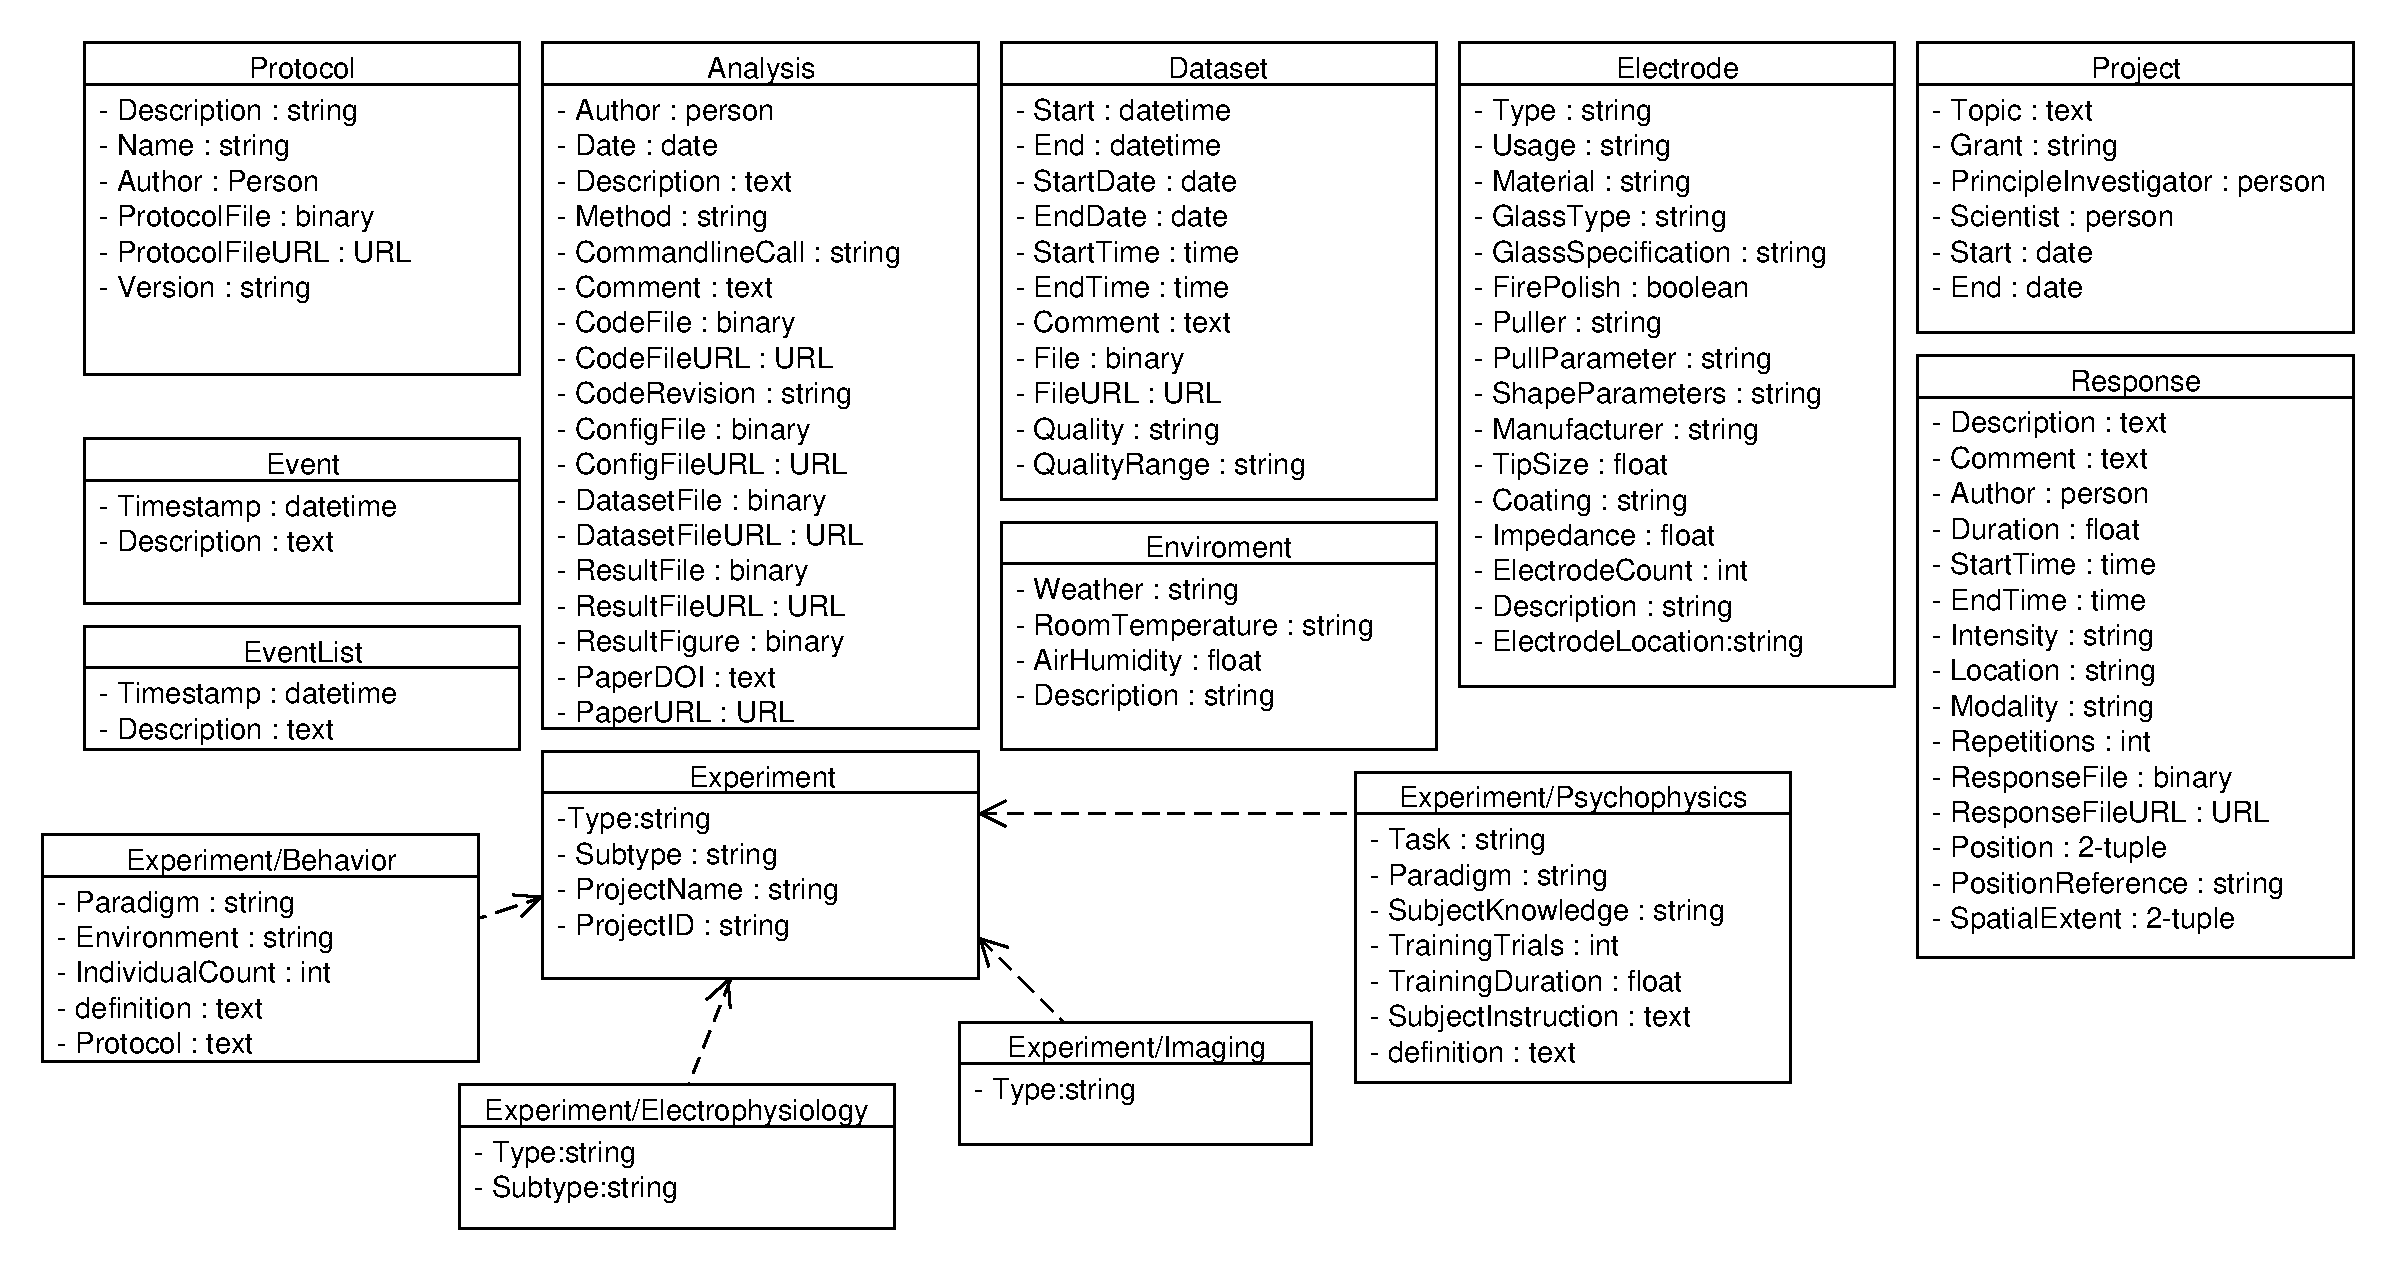
\includegraphics[scale=0.40]{obrazky/odml1.pdf}
		\caption{The \gls{odml}terminology. Part 1.}
		\label{meta_scheme1}
		
			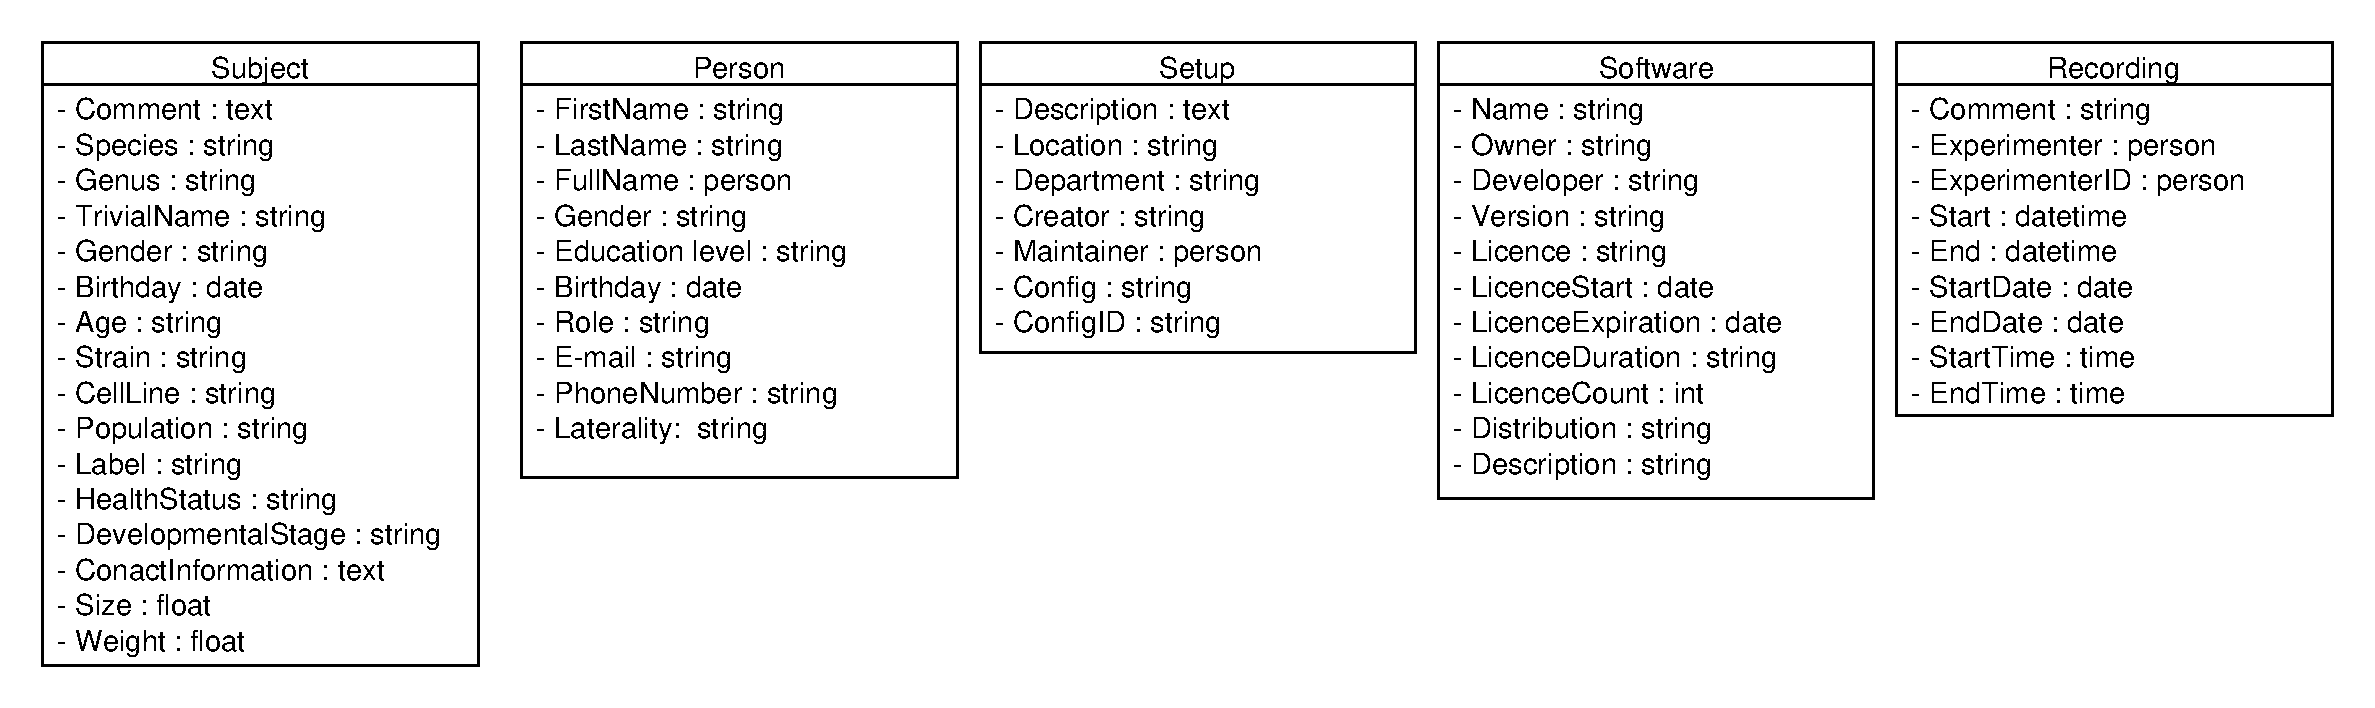
\includegraphics[scale=0.40]{obrazky/odml4.pdf}
			\caption{The \gls{odml}terminology. Part 2.}
			\label{meta_scheme2}
	\end{center}
\end{figure}

\begin{figure}[h]
	\begin{center}
		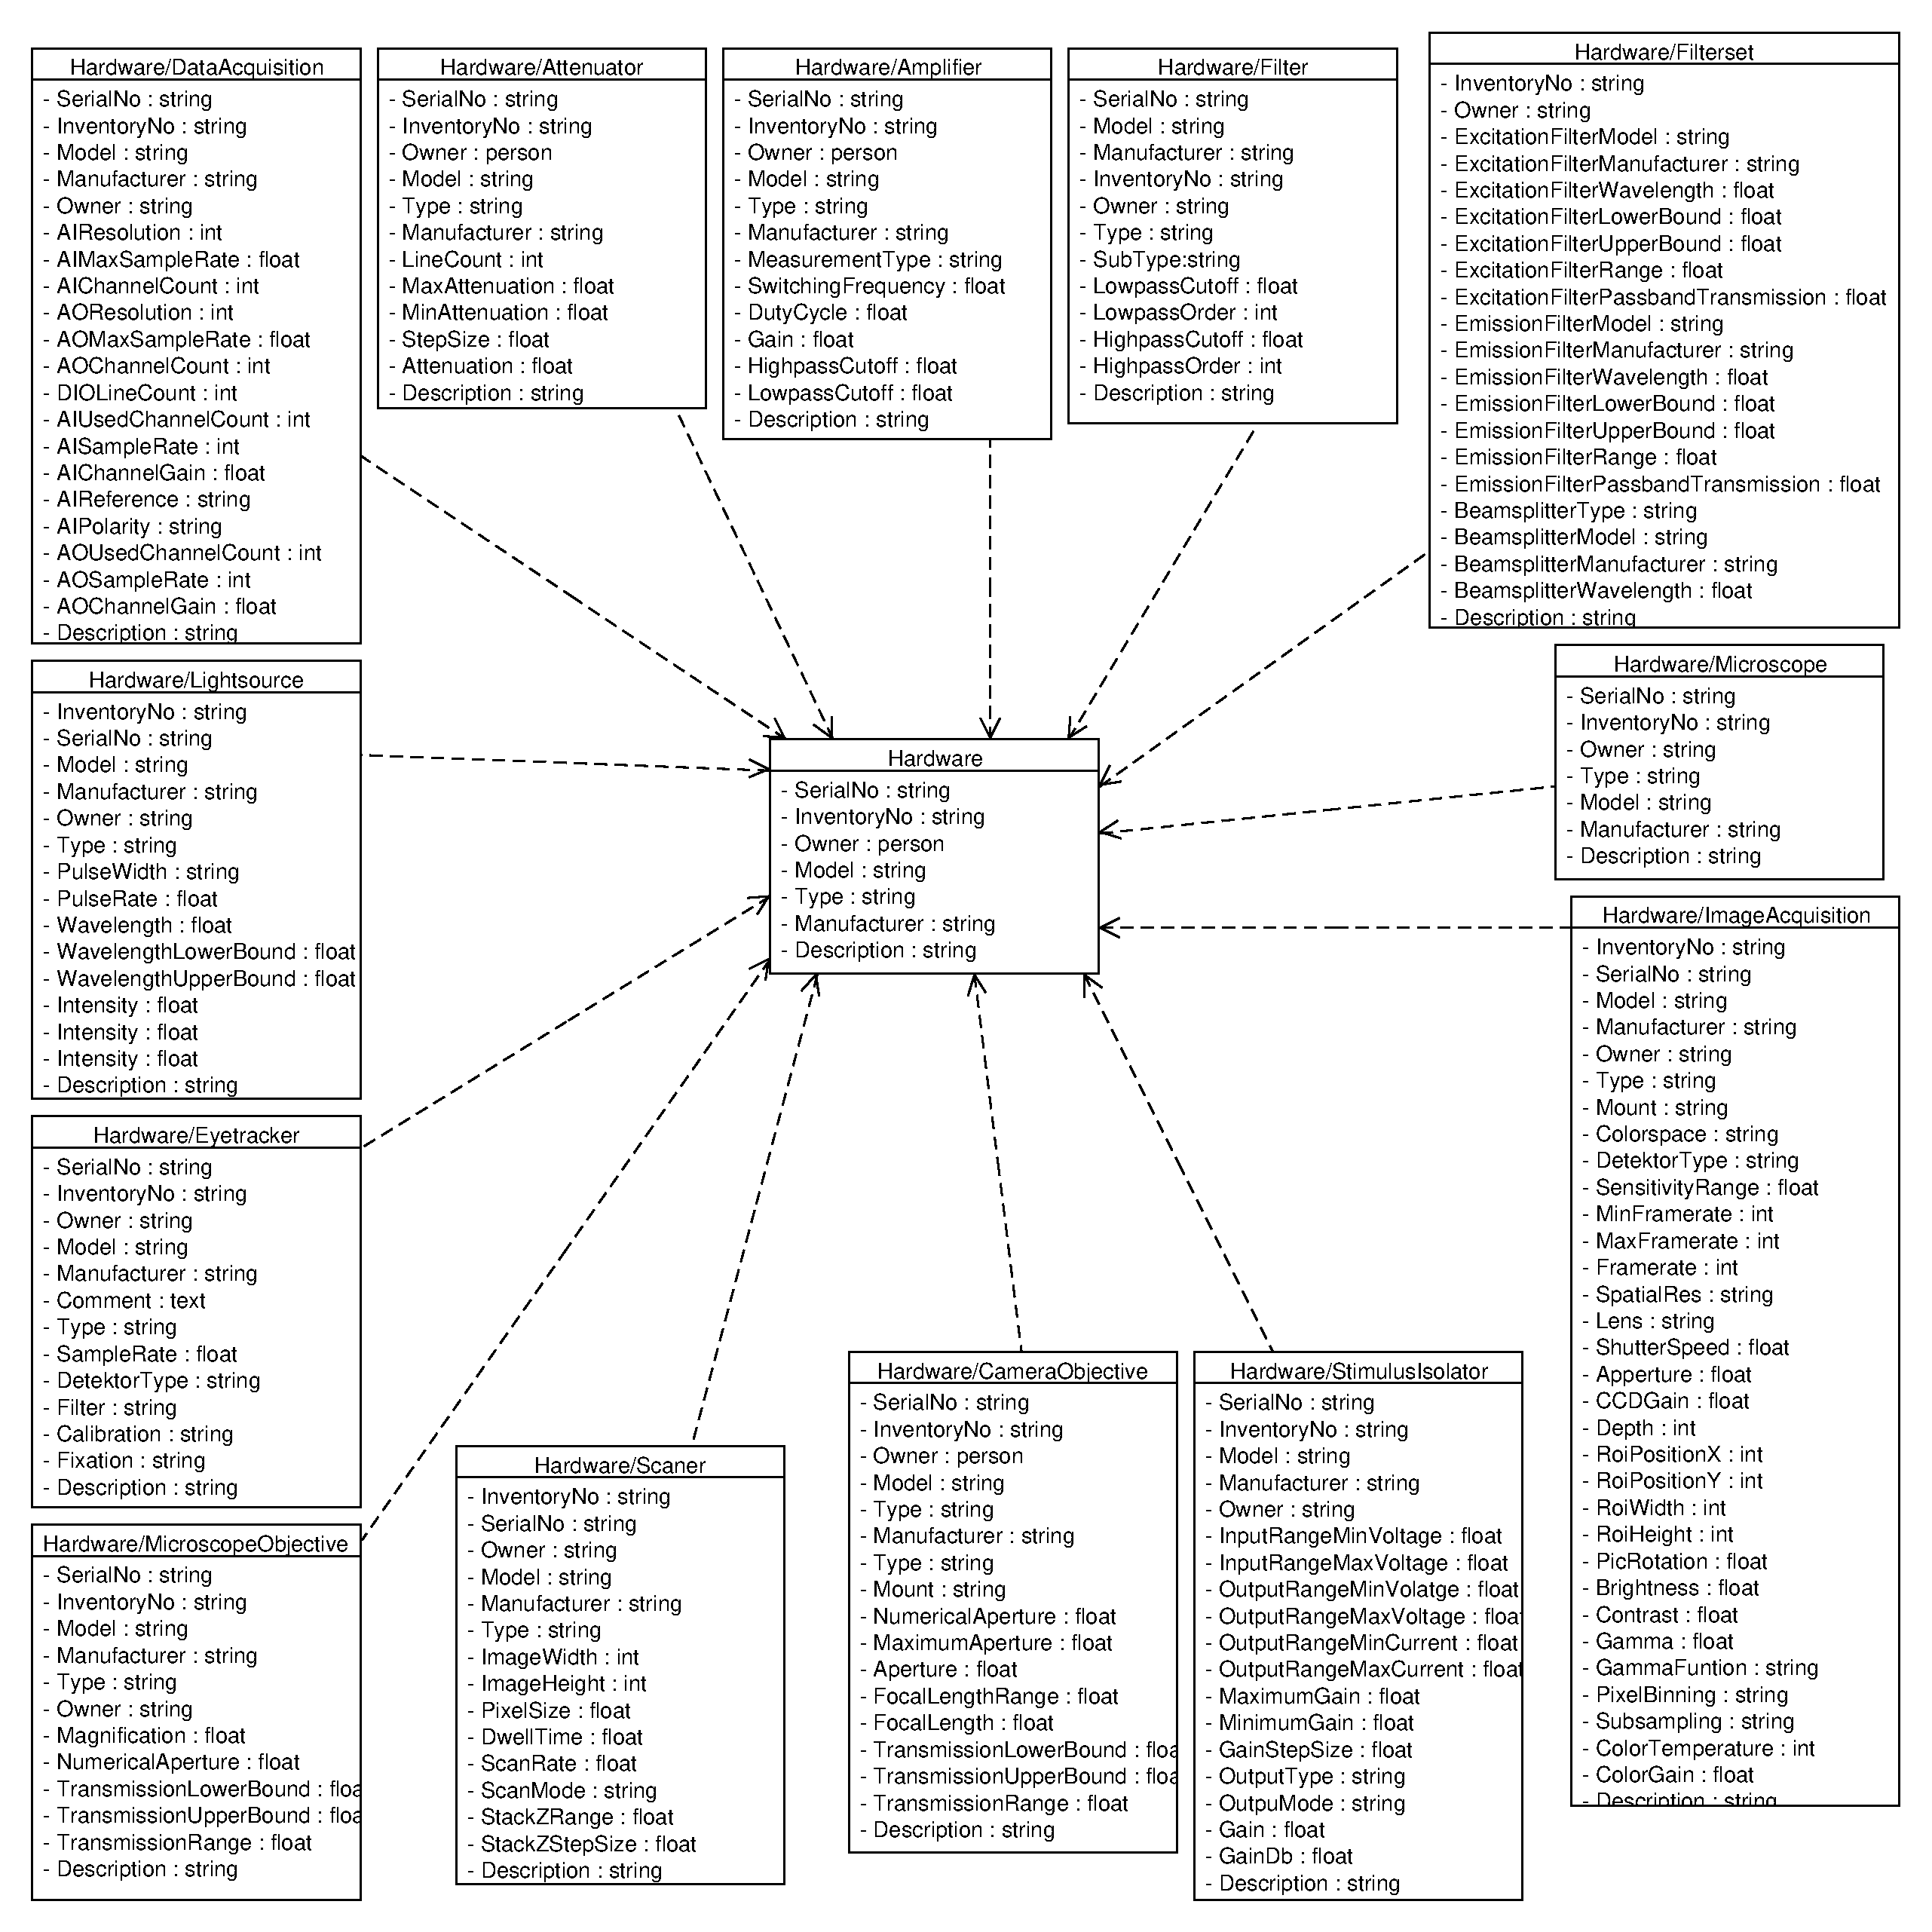
\includegraphics[scale=0.35]{obrazky/odml2.pdf}
		\caption{The \gls{odml}terminology. Part 3.}
		\label{meta_scheme3}
	\end{center}		
\end{figure}
\begin{figure}[h]
	\begin{center}		
		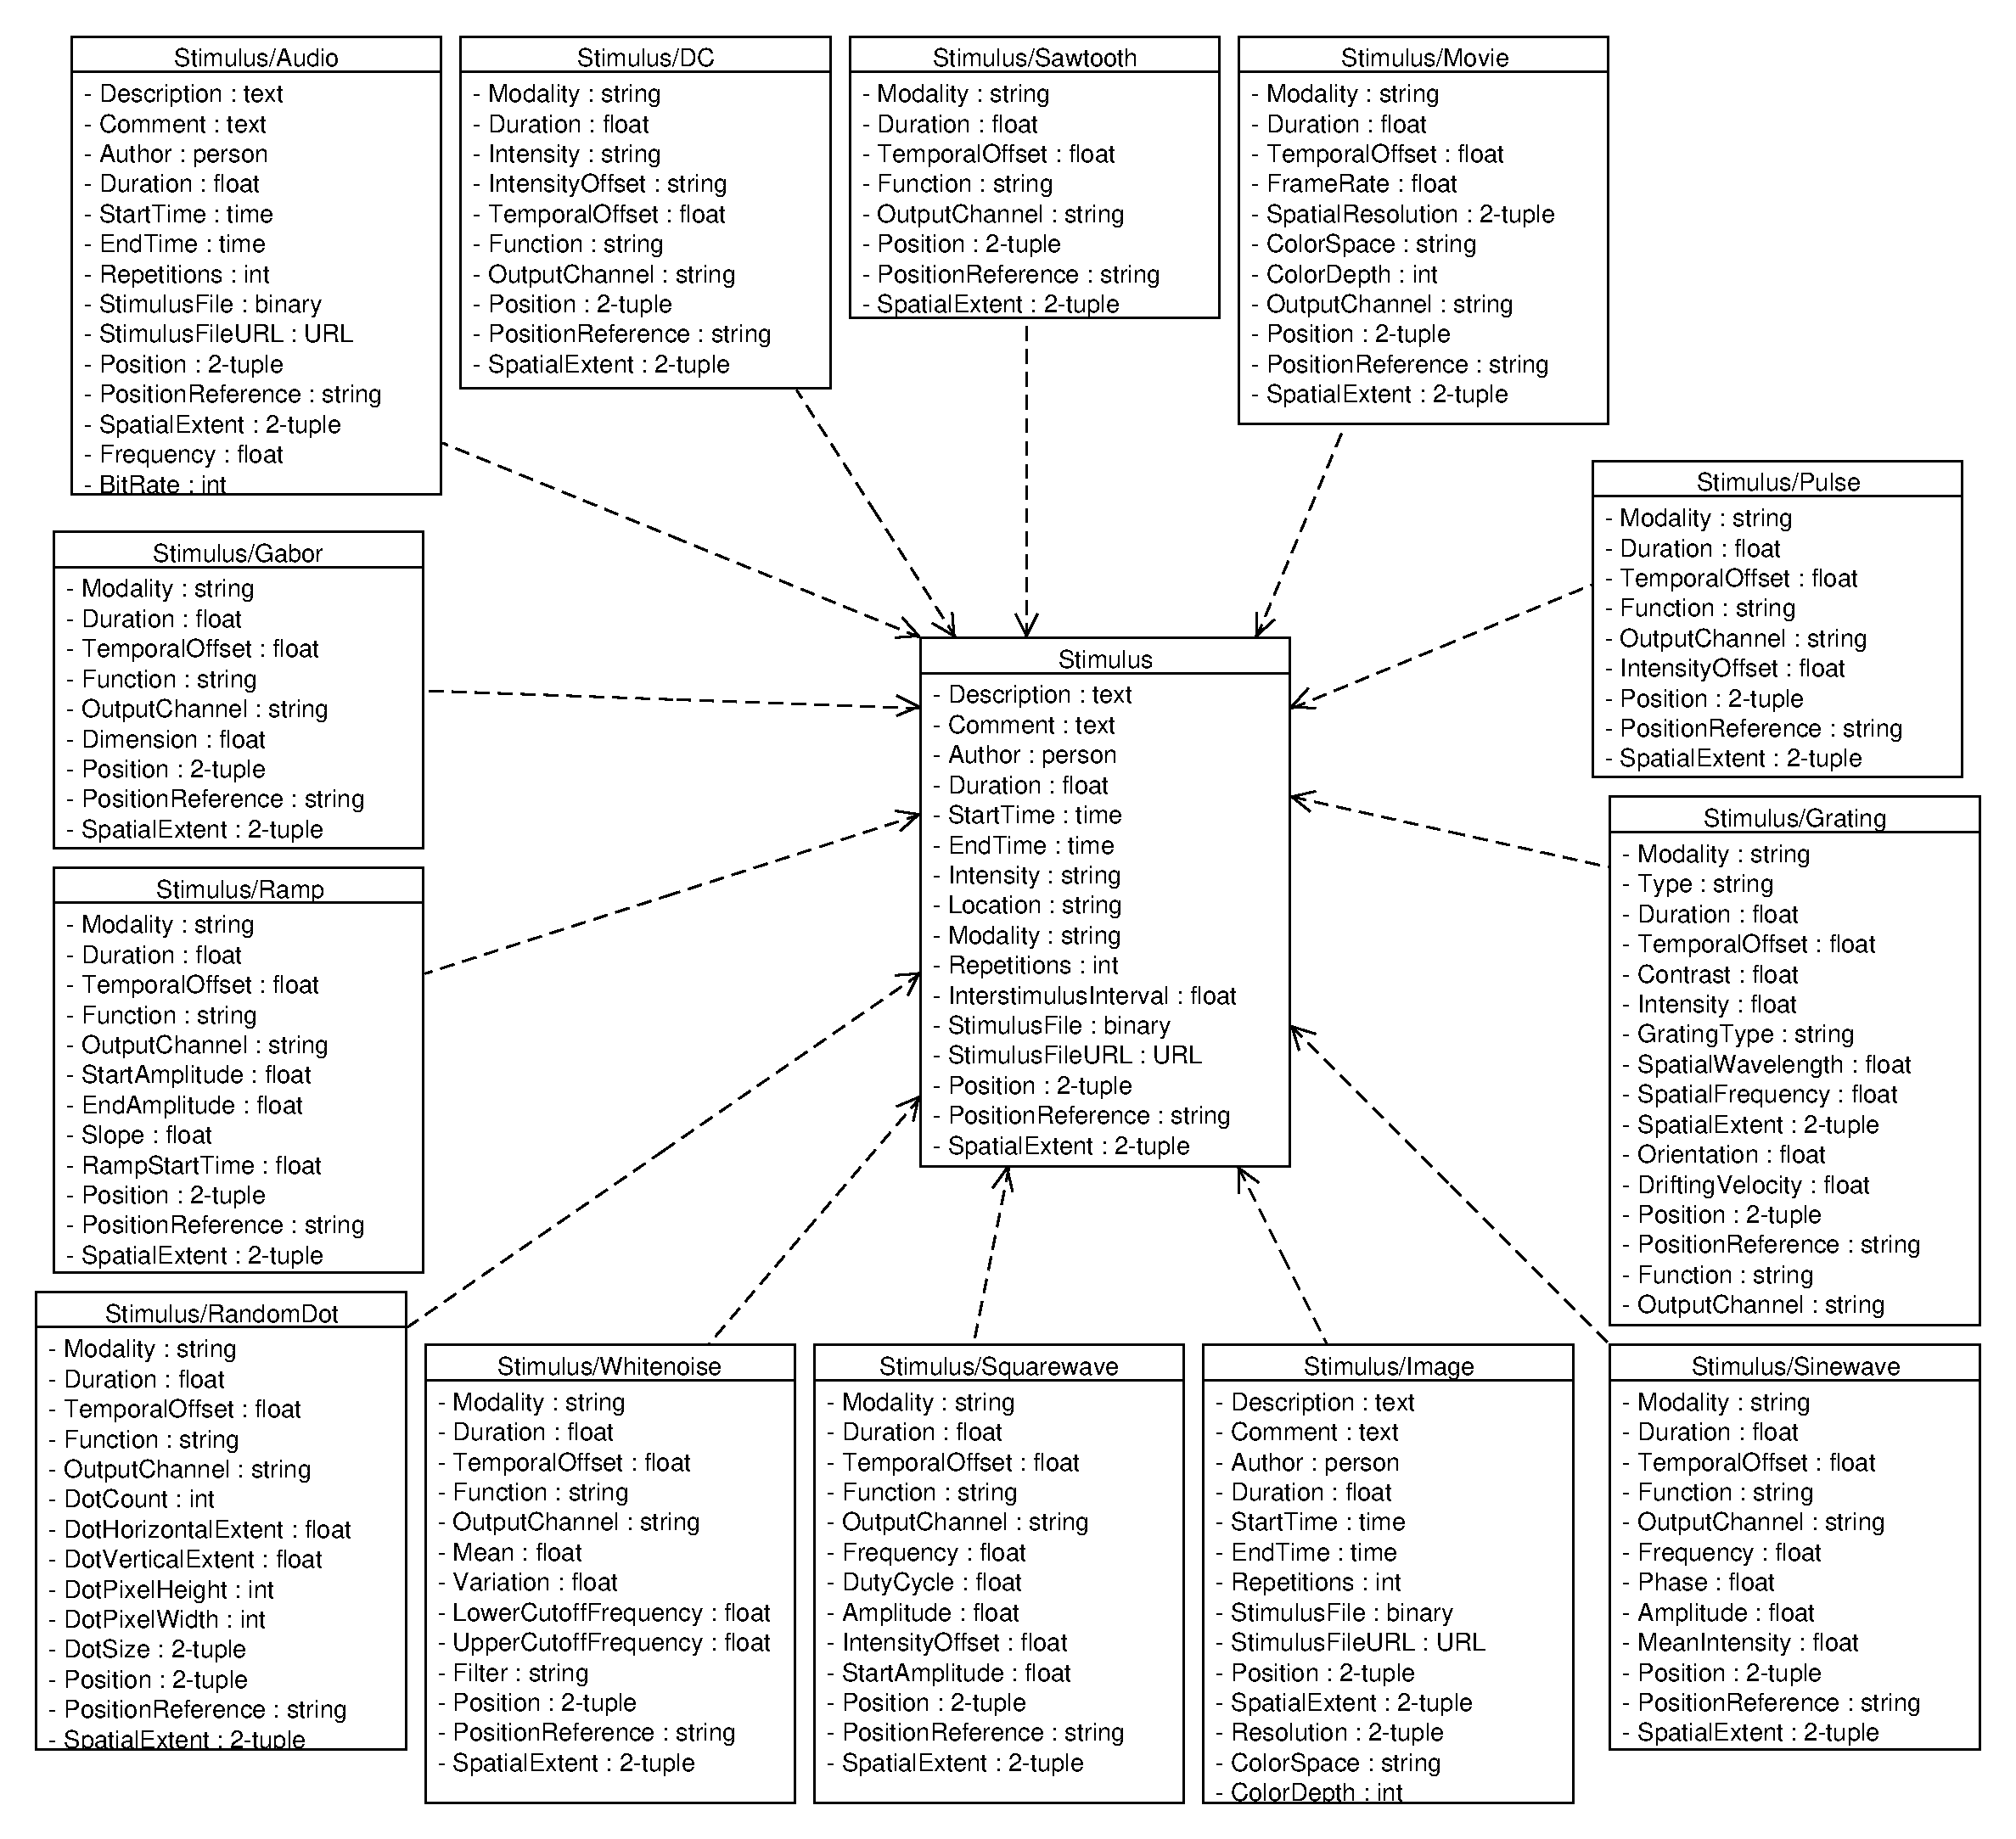
\includegraphics[scale=0.35]{obrazky/odml3.pdf}
		\caption{The \gls{odml}terminology. Part 4.}
		\label{meta_scheme4}
	\end{center}
\end{figure}

\chapter{Metadata Scheme}
\label{appendix2}
\begin{figure}[h]
	\begin{center}
		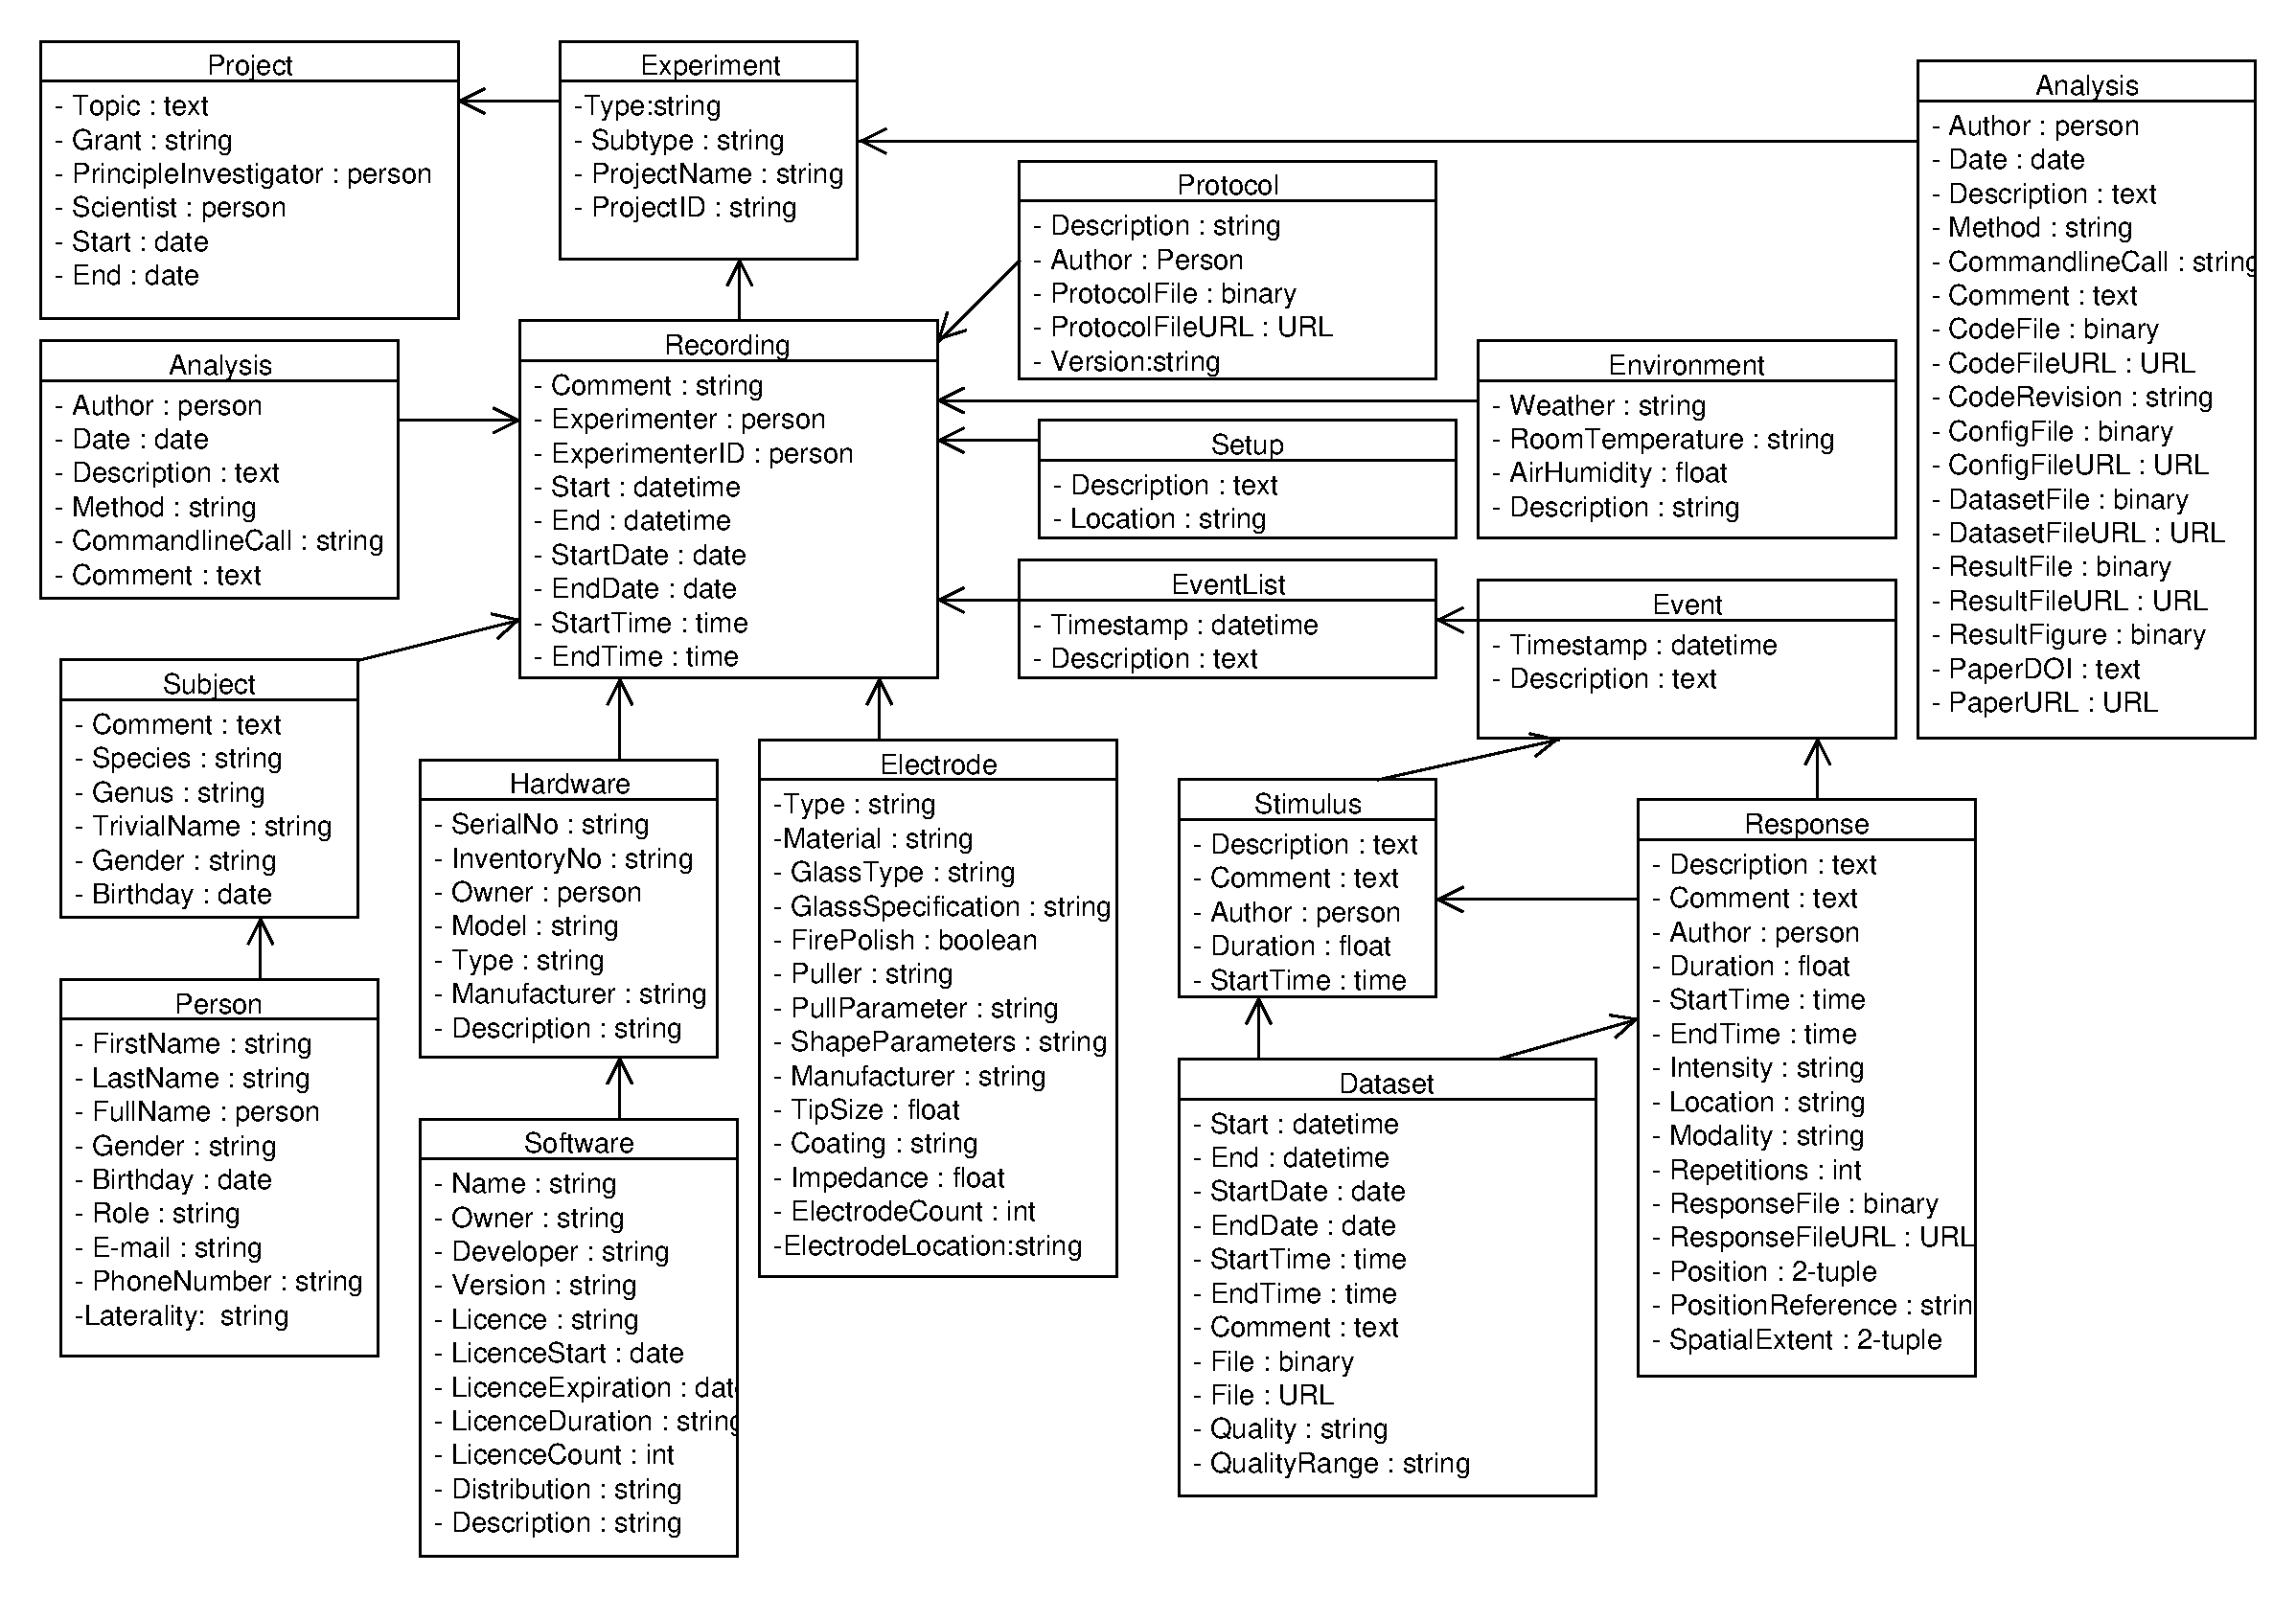
\includegraphics[scale=0.40]{obrazky/meta-scheme.pdf}
		\caption{Metadata scheme of EEGBase format.}
		\label{meta_scheme}
	\end{center}
\end{figure}

\chapter{Export Program User Manual}

\section{Installation}



The EEGExport program needs for its functionality installed HDF5 libraries version 2.10 or higher and Java Runtime Environment in version 1.7 or higher. The pre-build binary distribution could be obtained from official \href{https://www.hdfgroup.org/products/java/release/download.html\#download}{HDF Group website}. 

The EEGExport program do not require installation. Program is distributed as runnable jar and could be lunched with supplied "run.bat" file. \textbf{The path to installed HDF libraries must be in the bat file for the correct function filled.} (Listing~\ref{batfile}).

\begin{lstlisting}[language=C,frame=single,caption={Bat file},label=batfile]
@ECHO OFF
rem Fill in hdf_path path to installed HDF libraries
set hdf_path=C:\HDF_Group\HDF-JAVA\2.11.0\lib\jhdf5.dll
java -Dncsa.hdf.hdf5lib.H5.hdf5lib=%hdf_path% -jar program.jar
\end{lstlisting}

\section{Data Export}

The location of hvdr, eeg and vmrk files and exported files location and file name must be set before export. The load of eeg files from EEGBase portal is not working in current version. So the option 1 (Figure~\ref{prg_gui}) must be selected. 

\begin{figure}[h]
	\begin{center}		
		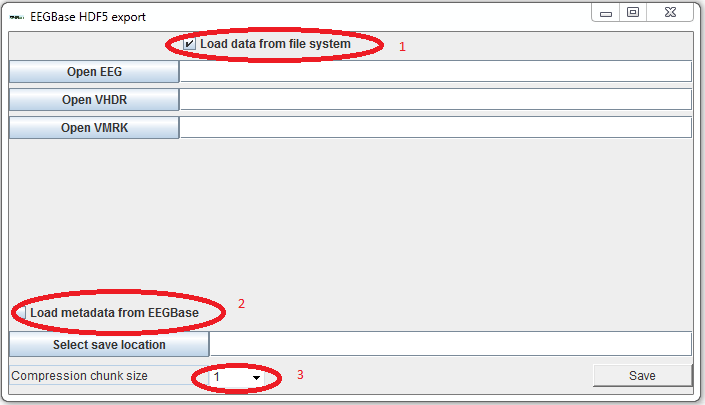
\includegraphics[scale=0.75]{obrazky/appendix/gui-start.png}
		\caption{The EEGExport program GUI}
		\label{prg_gui}
	\end{center}
\end{figure}
\newpage
\section{Metadata Export}

If the metadata from EEGBase portal should be exported as well the option 2 must be checked and the number of experiment must be filled (Figure~\ref{prg_meta}).

\section{Compression}

The final file size could be influenced by compression. The amount of compression is set by chunk size. The chunk size 1 means no compression. Bigger chunk size sets bigger compression so the file size is smaller.



\begin{figure}[h]
	\begin{center}		
		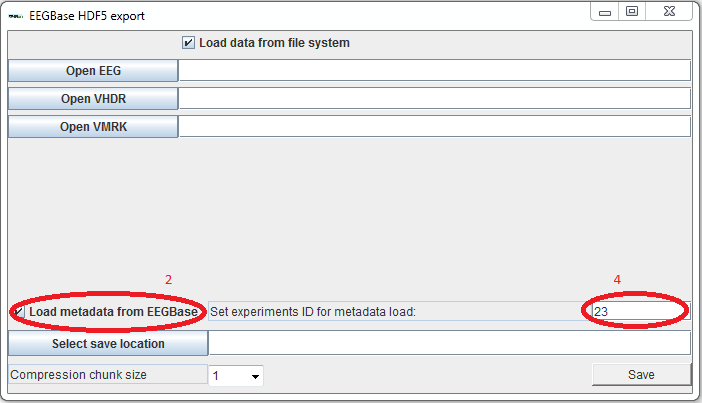
\includegraphics[scale=0.75]{obrazky/appendix/gui-meta.png}
		\caption{The EEGExport program GUI}
		\label{prg_meta}
	\end{center}
\end{figure}

\end{document}
